\chapter{Numerische Tests}
\label{cha:NumerischeTests}

In diesem Kapitel möchten wir die vorgestellten Verfahren verschiedenen numerischen Tests unterziehen. Dabei wollen wir hauptsächlich den Fehler der numerischen Lösung zur analytischen untersuchen, aber auch die Kondition der Kollokationsmatrizen, die Parameterwahl und die Laufzeit betrachten. Zusätzlich werden wir die Verfahren mit der finiten Elemente Methode (\acs{FEM}) vergleichen.

Dafür betrachten wir die Poisson-Gleichung mit Dirichlet-Randbedingung auf $\Omega = [-1,1] \times [-1,1] \subset \mathbb{R}^n$:
\begin{align*}
- \Delta u &= 2\pi^2 \sin(\pi x)\sin(\pi y)&&, (x,y) \in \Omega\\
u &= 0&&, (x,y) \in \partial \Omega
\end{align*}
mit analytischer Lösung $u(x,y) = \sin(\pi x)\sin(\pi y)$, dargestellt in Abbildung \ref{fig:plot}. Wir wählen als Gewichtsfunktion $w$ für $\Omega$ die Funktion aus Beispiel \ref{ex:Gewicht}:
\begin{align*}
w = -x^2-y^2+2 - \sqrt{x^4 -2x^2 + y^4 -2y^2+2}.
\end{align*}
\begin{figure}[h]
\centering
\resizebox {\columnwidth} {!} {
% This file was created by matlab2tikz.
%
%The latest updates can be retrieved from
%  http://www.mathworks.com/matlabcentral/fileexchange/22022-matlab2tikz-matlab2tikz
%where you can also make suggestions and rate matlab2tikz.
%
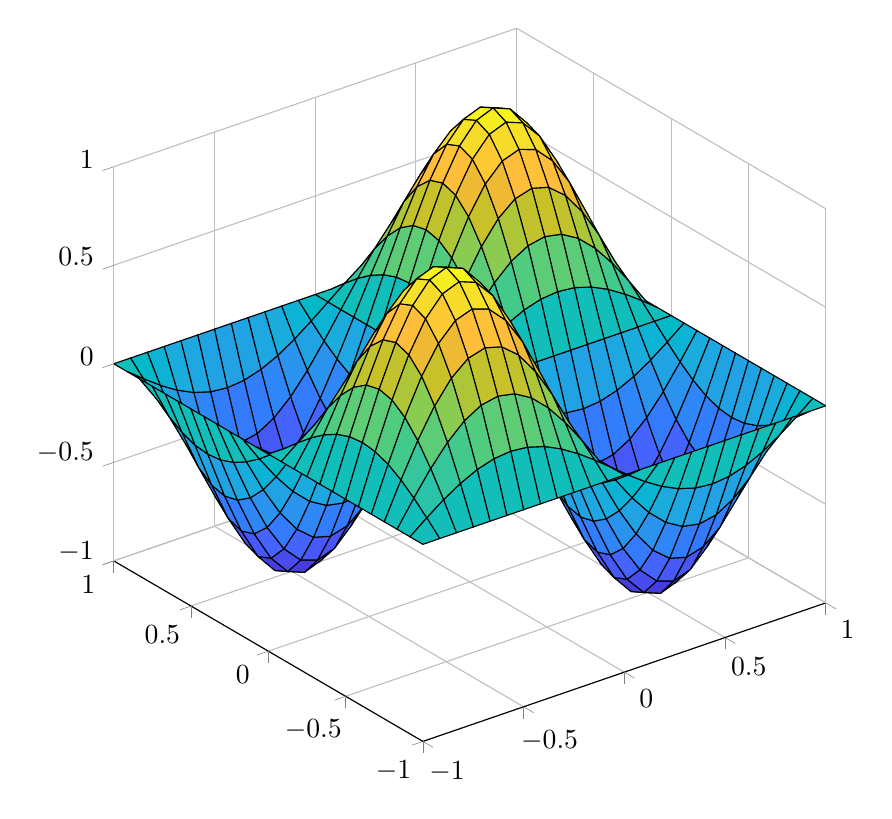
\begin{tikzpicture}

\begin{axis}[%
width=3.56in,
height=3.566in,
at={(0.597in,0.481in)},
scale only axis,
xmin=-1,
xmax=1,
tick align=outside,
ymin=-1,
ymax=1,
zmin=-1,
zmax=1,
view={-37.5}{30},
axis background/.style={fill=white},
axis x line*=bottom,
axis y line*=left,
axis z line*=left,
xmajorgrids,
ymajorgrids,
zmajorgrids,
legend style={at={(1.03,1)}, anchor=north west, legend cell align=left, align=left, draw=white!15!black}
]

\addplot3[%
surf,
shader=flat corner, draw=black, z buffer=sort, colormap={mymap}{[1pt] rgb(0pt)=(0.2422,0.1504,0.6603); rgb(1pt)=(0.25039,0.164995,0.707614); rgb(2pt)=(0.257771,0.181781,0.751138); rgb(3pt)=(0.264729,0.197757,0.795214); rgb(4pt)=(0.270648,0.214676,0.836371); rgb(5pt)=(0.275114,0.234238,0.870986); rgb(6pt)=(0.2783,0.255871,0.899071); rgb(7pt)=(0.280333,0.278233,0.9221); rgb(8pt)=(0.281338,0.300595,0.941376); rgb(9pt)=(0.281014,0.322757,0.957886); rgb(10pt)=(0.279467,0.344671,0.971676); rgb(11pt)=(0.275971,0.366681,0.982905); rgb(12pt)=(0.269914,0.3892,0.9906); rgb(13pt)=(0.260243,0.412329,0.995157); rgb(14pt)=(0.244033,0.435833,0.998833); rgb(15pt)=(0.220643,0.460257,0.997286); rgb(16pt)=(0.196333,0.484719,0.989152); rgb(17pt)=(0.183405,0.507371,0.979795); rgb(18pt)=(0.178643,0.528857,0.968157); rgb(19pt)=(0.176438,0.549905,0.952019); rgb(20pt)=(0.168743,0.570262,0.935871); rgb(21pt)=(0.154,0.5902,0.9218); rgb(22pt)=(0.146029,0.609119,0.907857); rgb(23pt)=(0.138024,0.627629,0.89729); rgb(24pt)=(0.124814,0.645929,0.888343); rgb(25pt)=(0.111252,0.6635,0.876314); rgb(26pt)=(0.0952095,0.679829,0.859781); rgb(27pt)=(0.0688714,0.694771,0.839357); rgb(28pt)=(0.0296667,0.708167,0.816333); rgb(29pt)=(0.00357143,0.720267,0.7917); rgb(30pt)=(0.00665714,0.731214,0.766014); rgb(31pt)=(0.0433286,0.741095,0.73941); rgb(32pt)=(0.0963952,0.75,0.712038); rgb(33pt)=(0.140771,0.7584,0.684157); rgb(34pt)=(0.1717,0.766962,0.655443); rgb(35pt)=(0.193767,0.775767,0.6251); rgb(36pt)=(0.216086,0.7843,0.5923); rgb(37pt)=(0.246957,0.791795,0.556743); rgb(38pt)=(0.290614,0.79729,0.518829); rgb(39pt)=(0.340643,0.8008,0.478857); rgb(40pt)=(0.3909,0.802871,0.435448); rgb(41pt)=(0.445629,0.802419,0.390919); rgb(42pt)=(0.5044,0.7993,0.348); rgb(43pt)=(0.561562,0.794233,0.304481); rgb(44pt)=(0.617395,0.787619,0.261238); rgb(45pt)=(0.671986,0.779271,0.2227); rgb(46pt)=(0.7242,0.769843,0.191029); rgb(47pt)=(0.773833,0.759805,0.16461); rgb(48pt)=(0.820314,0.749814,0.153529); rgb(49pt)=(0.863433,0.7406,0.159633); rgb(50pt)=(0.903543,0.733029,0.177414); rgb(51pt)=(0.939257,0.728786,0.209957); rgb(52pt)=(0.972757,0.729771,0.239443); rgb(53pt)=(0.995648,0.743371,0.237148); rgb(54pt)=(0.996986,0.765857,0.219943); rgb(55pt)=(0.995205,0.789252,0.202762); rgb(56pt)=(0.9892,0.813567,0.188533); rgb(57pt)=(0.978629,0.838629,0.176557); rgb(58pt)=(0.967648,0.8639,0.16429); rgb(59pt)=(0.96101,0.889019,0.153676); rgb(60pt)=(0.959671,0.913457,0.142257); rgb(61pt)=(0.962795,0.937338,0.12651); rgb(62pt)=(0.969114,0.960629,0.106362); rgb(63pt)=(0.9769,0.9839,0.0805)}, mesh/rows=25]
table[row sep=crcr, point meta=\thisrow{c}] {%
%
x	y	z	c\\
-1	-1	1.49975978266186e-32	1.49975978266186e-32\\
-0.916666666666667	-1	0	0\\
-0.833333333333333	-1	6.12323399573676e-17	6.12323399573676e-17\\
-0.75	-1	8.65956056235493e-17	8.65956056235493e-17\\
-0.666666666666667	-1	1.06057523872491e-16	1.06057523872491e-16\\
-0.583333333333333	-1	1.18291797137867e-16	1.18291797137867e-16\\
-0.5	-1	1.22464679914735e-16	1.22464679914735e-16\\
-0.416666666666667	-1	1.18291797137867e-16	1.18291797137867e-16\\
-0.333333333333333	-1	1.06057523872491e-16	1.06057523872491e-16\\
-0.25	-1	8.65956056235493e-17	8.65956056235493e-17\\
-0.166666666666667	-1	6.12323399573676e-17	6.12323399573676e-17\\
-0.0833333333333334	-1	3.16961915143177e-17	3.16961915143177e-17\\
0	-1	-0	-0\\
0.0833333333333333	-1	-3.16961915143176e-17	-3.16961915143176e-17\\
0.166666666666667	-1	-6.12323399573677e-17	-6.12323399573677e-17\\
0.25	-1	-8.65956056235493e-17	-8.65956056235493e-17\\
0.333333333333333	-1	-1.06057523872491e-16	-1.06057523872491e-16\\
0.416666666666667	-1	-1.18291797137867e-16	-1.18291797137867e-16\\
0.5	-1	-1.22464679914735e-16	-1.22464679914735e-16\\
0.583333333333333	-1	-1.18291797137867e-16	-1.18291797137867e-16\\
0.666666666666667	-1	-1.06057523872491e-16	-1.06057523872491e-16\\
0.75	-1	-8.65956056235493e-17	-8.65956056235493e-17\\
0.833333333333333	-1	-6.12323399573677e-17	-6.12323399573677e-17\\
0.916666666666667	-1	-3.16961915143176e-17	-3.16961915143176e-17\\
1	-1	-1.49975978266186e-32	-1.49975978266186e-32\\
-1	-0.916666666666667	3.16961915143177e-17	3.16961915143177e-17\\
-0.916666666666667	-0.916666666666667	0.0669872981077808	0.0669872981077808\\
-0.833333333333333	-0.916666666666667	0.12940952255126	0.12940952255126\\
-0.75	-0.916666666666667	0.18301270189222	0.18301270189222\\
-0.666666666666667	-0.916666666666667	0.224143868042014	0.224143868042014\\
-0.583333333333333	-0.916666666666667	0.25	0.25\\
-0.5	-0.916666666666667	0.258819045102521	0.258819045102521\\
-0.416666666666667	-0.916666666666667	0.25	0.25\\
-0.333333333333333	-0.916666666666667	0.224143868042014	0.224143868042014\\
-0.25	-0.916666666666667	0.183012701892219	0.183012701892219\\
-0.166666666666667	-0.916666666666667	0.12940952255126	0.12940952255126\\
-0.0833333333333334	-0.916666666666667	0.0669872981077808	0.0669872981077808\\
0	-0.916666666666667	-0	-0\\
0.0833333333333333	-0.916666666666667	-0.0669872981077807	-0.0669872981077807\\
0.166666666666667	-0.916666666666667	-0.129409522551261	-0.129409522551261\\
0.25	-0.916666666666667	-0.183012701892219	-0.183012701892219\\
0.333333333333333	-0.916666666666667	-0.224143868042014	-0.224143868042014\\
0.416666666666667	-0.916666666666667	-0.25	-0.25\\
0.5	-0.916666666666667	-0.258819045102521	-0.258819045102521\\
0.583333333333333	-0.916666666666667	-0.25	-0.25\\
0.666666666666667	-0.916666666666667	-0.224143868042014	-0.224143868042014\\
0.75	-0.916666666666667	-0.18301270189222	-0.18301270189222\\
0.833333333333333	-0.916666666666667	-0.129409522551261	-0.129409522551261\\
0.916666666666667	-0.916666666666667	-0.0669872981077807	-0.0669872981077807\\
1	-0.916666666666667	-3.16961915143177e-17	-3.16961915143177e-17\\
-1	-0.833333333333333	6.12323399573676e-17	6.12323399573676e-17\\
-0.916666666666667	-0.833333333333333	0.12940952255126	0.12940952255126\\
-0.833333333333333	-0.833333333333333	0.25	0.25\\
-0.75	-0.833333333333333	0.353553390593274	0.353553390593274\\
-0.666666666666667	-0.833333333333333	0.433012701892219	0.433012701892219\\
-0.583333333333333	-0.833333333333333	0.482962913144534	0.482962913144534\\
-0.5	-0.833333333333333	0.5	0.5\\
-0.416666666666667	-0.833333333333333	0.482962913144534	0.482962913144534\\
-0.333333333333333	-0.833333333333333	0.433012701892219	0.433012701892219\\
-0.25	-0.833333333333333	0.353553390593274	0.353553390593274\\
-0.166666666666667	-0.833333333333333	0.25	0.25\\
-0.0833333333333334	-0.833333333333333	0.12940952255126	0.12940952255126\\
0	-0.833333333333333	-0	-0\\
0.0833333333333333	-0.833333333333333	-0.12940952255126	-0.12940952255126\\
0.166666666666667	-0.833333333333333	-0.25	-0.25\\
0.25	-0.833333333333333	-0.353553390593274	-0.353553390593274\\
0.333333333333333	-0.833333333333333	-0.433012701892219	-0.433012701892219\\
0.416666666666667	-0.833333333333333	-0.482962913144534	-0.482962913144534\\
0.5	-0.833333333333333	-0.5	-0.5\\
0.583333333333333	-0.833333333333333	-0.482962913144534	-0.482962913144534\\
0.666666666666667	-0.833333333333333	-0.433012701892219	-0.433012701892219\\
0.75	-0.833333333333333	-0.353553390593274	-0.353553390593274\\
0.833333333333333	-0.833333333333333	-0.25	-0.25\\
0.916666666666667	-0.833333333333333	-0.12940952255126	-0.12940952255126\\
1	-0.833333333333333	-6.12323399573676e-17	-6.12323399573676e-17\\
-1	-0.75	8.65956056235493e-17	8.65956056235493e-17\\
-0.916666666666667	-0.75	0.18301270189222	0.18301270189222\\
-0.833333333333333	-0.75	0.353553390593274	0.353553390593274\\
-0.75	-0.75	0.5	0.5\\
-0.666666666666667	-0.75	0.612372435695795	0.612372435695795\\
-0.583333333333333	-0.75	0.68301270189222	0.68301270189222\\
-0.5	-0.75	0.707106781186548	0.707106781186548\\
-0.416666666666667	-0.75	0.683012701892219	0.683012701892219\\
-0.333333333333333	-0.75	0.612372435695795	0.612372435695795\\
-0.25	-0.75	0.5	0.5\\
-0.166666666666667	-0.75	0.353553390593274	0.353553390593274\\
-0.0833333333333334	-0.75	0.183012701892219	0.183012701892219\\
0	-0.75	-0	-0\\
0.0833333333333333	-0.75	-0.183012701892219	-0.183012701892219\\
0.166666666666667	-0.75	-0.353553390593274	-0.353553390593274\\
0.25	-0.75	-0.5	-0.5\\
0.333333333333333	-0.75	-0.612372435695794	-0.612372435695794\\
0.416666666666667	-0.75	-0.683012701892219	-0.683012701892219\\
0.5	-0.75	-0.707106781186548	-0.707106781186548\\
0.583333333333333	-0.75	-0.68301270189222	-0.68301270189222\\
0.666666666666667	-0.75	-0.612372435695795	-0.612372435695795\\
0.75	-0.75	-0.5	-0.5\\
0.833333333333333	-0.75	-0.353553390593274	-0.353553390593274\\
0.916666666666667	-0.75	-0.183012701892219	-0.183012701892219\\
1	-0.75	-8.65956056235493e-17	-8.65956056235493e-17\\
-1	-0.666666666666667	1.06057523872491e-16	1.06057523872491e-16\\
-0.916666666666667	-0.666666666666667	0.224143868042014	0.224143868042014\\
-0.833333333333333	-0.666666666666667	0.433012701892219	0.433012701892219\\
-0.75	-0.666666666666667	0.612372435695795	0.612372435695795\\
-0.666666666666667	-0.666666666666667	0.75	0.75\\
-0.583333333333333	-0.666666666666667	0.836516303737808	0.836516303737808\\
-0.5	-0.666666666666667	0.866025403784439	0.866025403784439\\
-0.416666666666667	-0.666666666666667	0.836516303737808	0.836516303737808\\
-0.333333333333333	-0.666666666666667	0.75	0.75\\
-0.25	-0.666666666666667	0.612372435695794	0.612372435695794\\
-0.166666666666667	-0.666666666666667	0.433012701892219	0.433012701892219\\
-0.0833333333333334	-0.666666666666667	0.224143868042013	0.224143868042013\\
0	-0.666666666666667	-0	-0\\
0.0833333333333333	-0.666666666666667	-0.224143868042013	-0.224143868042013\\
0.166666666666667	-0.666666666666667	-0.433012701892219	-0.433012701892219\\
0.25	-0.666666666666667	-0.612372435695794	-0.612372435695794\\
0.333333333333333	-0.666666666666667	-0.75	-0.75\\
0.416666666666667	-0.666666666666667	-0.836516303737808	-0.836516303737808\\
0.5	-0.666666666666667	-0.866025403784439	-0.866025403784439\\
0.583333333333333	-0.666666666666667	-0.836516303737808	-0.836516303737808\\
0.666666666666667	-0.666666666666667	-0.75	-0.75\\
0.75	-0.666666666666667	-0.612372435695795	-0.612372435695795\\
0.833333333333333	-0.666666666666667	-0.43301270189222	-0.43301270189222\\
0.916666666666667	-0.666666666666667	-0.224143868042013	-0.224143868042013\\
1	-0.666666666666667	-1.06057523872491e-16	-1.06057523872491e-16\\
-1	-0.583333333333333	1.18291797137867e-16	1.18291797137867e-16\\
-0.916666666666667	-0.583333333333333	0.25	0.25\\
-0.833333333333333	-0.583333333333333	0.482962913144534	0.482962913144534\\
-0.75	-0.583333333333333	0.68301270189222	0.68301270189222\\
-0.666666666666667	-0.583333333333333	0.836516303737808	0.836516303737808\\
-0.583333333333333	-0.583333333333333	0.93301270189222	0.93301270189222\\
-0.5	-0.583333333333333	0.965925826289068	0.965925826289068\\
-0.416666666666667	-0.583333333333333	0.933012701892219	0.933012701892219\\
-0.333333333333333	-0.583333333333333	0.836516303737808	0.836516303737808\\
-0.25	-0.583333333333333	0.683012701892219	0.683012701892219\\
-0.166666666666667	-0.583333333333333	0.482962913144534	0.482962913144534\\
-0.0833333333333334	-0.583333333333333	0.25	0.25\\
0	-0.583333333333333	-0	-0\\
0.0833333333333333	-0.583333333333333	-0.25	-0.25\\
0.166666666666667	-0.583333333333333	-0.482962913144534	-0.482962913144534\\
0.25	-0.583333333333333	-0.683012701892219	-0.683012701892219\\
0.333333333333333	-0.583333333333333	-0.836516303737808	-0.836516303737808\\
0.416666666666667	-0.583333333333333	-0.93301270189222	-0.93301270189222\\
0.5	-0.583333333333333	-0.965925826289068	-0.965925826289068\\
0.583333333333333	-0.583333333333333	-0.93301270189222	-0.93301270189222\\
0.666666666666667	-0.583333333333333	-0.836516303737808	-0.836516303737808\\
0.75	-0.583333333333333	-0.68301270189222	-0.68301270189222\\
0.833333333333333	-0.583333333333333	-0.482962913144535	-0.482962913144535\\
0.916666666666667	-0.583333333333333	-0.25	-0.25\\
1	-0.583333333333333	-1.18291797137867e-16	-1.18291797137867e-16\\
-1	-0.5	1.22464679914735e-16	1.22464679914735e-16\\
-0.916666666666667	-0.5	0.258819045102521	0.258819045102521\\
-0.833333333333333	-0.5	0.5	0.5\\
-0.75	-0.5	0.707106781186548	0.707106781186548\\
-0.666666666666667	-0.5	0.866025403784439	0.866025403784439\\
-0.583333333333333	-0.5	0.965925826289068	0.965925826289068\\
-0.5	-0.5	1	1\\
-0.416666666666667	-0.5	0.965925826289068	0.965925826289068\\
-0.333333333333333	-0.5	0.866025403784439	0.866025403784439\\
-0.25	-0.5	0.707106781186547	0.707106781186547\\
-0.166666666666667	-0.5	0.5	0.5\\
-0.0833333333333334	-0.5	0.258819045102521	0.258819045102521\\
0	-0.5	-0	-0\\
0.0833333333333333	-0.5	-0.258819045102521	-0.258819045102521\\
0.166666666666667	-0.5	-0.5	-0.5\\
0.25	-0.5	-0.707106781186547	-0.707106781186547\\
0.333333333333333	-0.5	-0.866025403784438	-0.866025403784438\\
0.416666666666667	-0.5	-0.965925826289068	-0.965925826289068\\
0.5	-0.5	-1	-1\\
0.583333333333333	-0.5	-0.965925826289068	-0.965925826289068\\
0.666666666666667	-0.5	-0.866025403784439	-0.866025403784439\\
0.75	-0.5	-0.707106781186548	-0.707106781186548\\
0.833333333333333	-0.5	-0.5	-0.5\\
0.916666666666667	-0.5	-0.258819045102521	-0.258819045102521\\
1	-0.5	-1.22464679914735e-16	-1.22464679914735e-16\\
-1	-0.416666666666667	1.18291797137867e-16	1.18291797137867e-16\\
-0.916666666666667	-0.416666666666667	0.25	0.25\\
-0.833333333333333	-0.416666666666667	0.482962913144534	0.482962913144534\\
-0.75	-0.416666666666667	0.683012701892219	0.683012701892219\\
-0.666666666666667	-0.416666666666667	0.836516303737808	0.836516303737808\\
-0.583333333333333	-0.416666666666667	0.933012701892219	0.933012701892219\\
-0.5	-0.416666666666667	0.965925826289068	0.965925826289068\\
-0.416666666666667	-0.416666666666667	0.933012701892219	0.933012701892219\\
-0.333333333333333	-0.416666666666667	0.836516303737808	0.836516303737808\\
-0.25	-0.416666666666667	0.683012701892219	0.683012701892219\\
-0.166666666666667	-0.416666666666667	0.482962913144534	0.482962913144534\\
-0.0833333333333334	-0.416666666666667	0.25	0.25\\
0	-0.416666666666667	-0	-0\\
0.0833333333333333	-0.416666666666667	-0.25	-0.25\\
0.166666666666667	-0.416666666666667	-0.482962913144534	-0.482962913144534\\
0.25	-0.416666666666667	-0.683012701892219	-0.683012701892219\\
0.333333333333333	-0.416666666666667	-0.836516303737808	-0.836516303737808\\
0.416666666666667	-0.416666666666667	-0.933012701892219	-0.933012701892219\\
0.5	-0.416666666666667	-0.965925826289068	-0.965925826289068\\
0.583333333333333	-0.416666666666667	-0.933012701892219	-0.933012701892219\\
0.666666666666667	-0.416666666666667	-0.836516303737808	-0.836516303737808\\
0.75	-0.416666666666667	-0.683012701892219	-0.683012701892219\\
0.833333333333333	-0.416666666666667	-0.482962913144534	-0.482962913144534\\
0.916666666666667	-0.416666666666667	-0.25	-0.25\\
1	-0.416666666666667	-1.18291797137867e-16	-1.18291797137867e-16\\
-1	-0.333333333333333	1.06057523872491e-16	1.06057523872491e-16\\
-0.916666666666667	-0.333333333333333	0.224143868042014	0.224143868042014\\
-0.833333333333333	-0.333333333333333	0.433012701892219	0.433012701892219\\
-0.75	-0.333333333333333	0.612372435695795	0.612372435695795\\
-0.666666666666667	-0.333333333333333	0.75	0.75\\
-0.583333333333333	-0.333333333333333	0.836516303737808	0.836516303737808\\
-0.5	-0.333333333333333	0.866025403784439	0.866025403784439\\
-0.416666666666667	-0.333333333333333	0.836516303737808	0.836516303737808\\
-0.333333333333333	-0.333333333333333	0.75	0.75\\
-0.25	-0.333333333333333	0.612372435695794	0.612372435695794\\
-0.166666666666667	-0.333333333333333	0.433012701892219	0.433012701892219\\
-0.0833333333333334	-0.333333333333333	0.224143868042013	0.224143868042013\\
0	-0.333333333333333	-0	-0\\
0.0833333333333333	-0.333333333333333	-0.224143868042013	-0.224143868042013\\
0.166666666666667	-0.333333333333333	-0.433012701892219	-0.433012701892219\\
0.25	-0.333333333333333	-0.612372435695794	-0.612372435695794\\
0.333333333333333	-0.333333333333333	-0.75	-0.75\\
0.416666666666667	-0.333333333333333	-0.836516303737808	-0.836516303737808\\
0.5	-0.333333333333333	-0.866025403784439	-0.866025403784439\\
0.583333333333333	-0.333333333333333	-0.836516303737808	-0.836516303737808\\
0.666666666666667	-0.333333333333333	-0.75	-0.75\\
0.75	-0.333333333333333	-0.612372435695795	-0.612372435695795\\
0.833333333333333	-0.333333333333333	-0.43301270189222	-0.43301270189222\\
0.916666666666667	-0.333333333333333	-0.224143868042013	-0.224143868042013\\
1	-0.333333333333333	-1.06057523872491e-16	-1.06057523872491e-16\\
-1	-0.25	8.65956056235493e-17	8.65956056235493e-17\\
-0.916666666666667	-0.25	0.183012701892219	0.183012701892219\\
-0.833333333333333	-0.25	0.353553390593274	0.353553390593274\\
-0.75	-0.25	0.5	0.5\\
-0.666666666666667	-0.25	0.612372435695794	0.612372435695794\\
-0.583333333333333	-0.25	0.683012701892219	0.683012701892219\\
-0.5	-0.25	0.707106781186547	0.707106781186547\\
-0.416666666666667	-0.25	0.683012701892219	0.683012701892219\\
-0.333333333333333	-0.25	0.612372435695794	0.612372435695794\\
-0.25	-0.25	0.5	0.5\\
-0.166666666666667	-0.25	0.353553390593274	0.353553390593274\\
-0.0833333333333334	-0.25	0.183012701892219	0.183012701892219\\
0	-0.25	-0	-0\\
0.0833333333333333	-0.25	-0.183012701892219	-0.183012701892219\\
0.166666666666667	-0.25	-0.353553390593274	-0.353553390593274\\
0.25	-0.25	-0.5	-0.5\\
0.333333333333333	-0.25	-0.612372435695794	-0.612372435695794\\
0.416666666666667	-0.25	-0.683012701892219	-0.683012701892219\\
0.5	-0.25	-0.707106781186547	-0.707106781186547\\
0.583333333333333	-0.25	-0.683012701892219	-0.683012701892219\\
0.666666666666667	-0.25	-0.612372435695794	-0.612372435695794\\
0.75	-0.25	-0.5	-0.5\\
0.833333333333333	-0.25	-0.353553390593274	-0.353553390593274\\
0.916666666666667	-0.25	-0.183012701892219	-0.183012701892219\\
1	-0.25	-8.65956056235493e-17	-8.65956056235493e-17\\
-1	-0.166666666666667	6.12323399573676e-17	6.12323399573676e-17\\
-0.916666666666667	-0.166666666666667	0.12940952255126	0.12940952255126\\
-0.833333333333333	-0.166666666666667	0.25	0.25\\
-0.75	-0.166666666666667	0.353553390593274	0.353553390593274\\
-0.666666666666667	-0.166666666666667	0.433012701892219	0.433012701892219\\
-0.583333333333333	-0.166666666666667	0.482962913144534	0.482962913144534\\
-0.5	-0.166666666666667	0.5	0.5\\
-0.416666666666667	-0.166666666666667	0.482962913144534	0.482962913144534\\
-0.333333333333333	-0.166666666666667	0.433012701892219	0.433012701892219\\
-0.25	-0.166666666666667	0.353553390593274	0.353553390593274\\
-0.166666666666667	-0.166666666666667	0.25	0.25\\
-0.0833333333333334	-0.166666666666667	0.12940952255126	0.12940952255126\\
0	-0.166666666666667	-0	-0\\
0.0833333333333333	-0.166666666666667	-0.12940952255126	-0.12940952255126\\
0.166666666666667	-0.166666666666667	-0.25	-0.25\\
0.25	-0.166666666666667	-0.353553390593274	-0.353553390593274\\
0.333333333333333	-0.166666666666667	-0.433012701892219	-0.433012701892219\\
0.416666666666667	-0.166666666666667	-0.482962913144534	-0.482962913144534\\
0.5	-0.166666666666667	-0.5	-0.5\\
0.583333333333333	-0.166666666666667	-0.482962913144534	-0.482962913144534\\
0.666666666666667	-0.166666666666667	-0.433012701892219	-0.433012701892219\\
0.75	-0.166666666666667	-0.353553390593274	-0.353553390593274\\
0.833333333333333	-0.166666666666667	-0.25	-0.25\\
0.916666666666667	-0.166666666666667	-0.12940952255126	-0.12940952255126\\
1	-0.166666666666667	-6.12323399573676e-17	-6.12323399573676e-17\\
-1	-0.0833333333333334	3.16961915143177e-17	3.16961915143177e-17\\
-0.916666666666667	-0.0833333333333334	0.0669872981077808	0.0669872981077808\\
-0.833333333333333	-0.0833333333333334	0.12940952255126	0.12940952255126\\
-0.75	-0.0833333333333334	0.183012701892219	0.183012701892219\\
-0.666666666666667	-0.0833333333333334	0.224143868042013	0.224143868042013\\
-0.583333333333333	-0.0833333333333334	0.25	0.25\\
-0.5	-0.0833333333333334	0.258819045102521	0.258819045102521\\
-0.416666666666667	-0.0833333333333334	0.25	0.25\\
-0.333333333333333	-0.0833333333333334	0.224143868042013	0.224143868042013\\
-0.25	-0.0833333333333334	0.183012701892219	0.183012701892219\\
-0.166666666666667	-0.0833333333333334	0.12940952255126	0.12940952255126\\
-0.0833333333333334	-0.0833333333333334	0.0669872981077807	0.0669872981077807\\
0	-0.0833333333333334	-0	-0\\
0.0833333333333333	-0.0833333333333334	-0.0669872981077806	-0.0669872981077806\\
0.166666666666667	-0.0833333333333334	-0.12940952255126	-0.12940952255126\\
0.25	-0.0833333333333334	-0.183012701892219	-0.183012701892219\\
0.333333333333333	-0.0833333333333334	-0.224143868042013	-0.224143868042013\\
0.416666666666667	-0.0833333333333334	-0.25	-0.25\\
0.5	-0.0833333333333334	-0.258819045102521	-0.258819045102521\\
0.583333333333333	-0.0833333333333334	-0.25	-0.25\\
0.666666666666667	-0.0833333333333334	-0.224143868042013	-0.224143868042013\\
0.75	-0.0833333333333334	-0.183012701892219	-0.183012701892219\\
0.833333333333333	-0.0833333333333334	-0.129409522551261	-0.129409522551261\\
0.916666666666667	-0.0833333333333334	-0.0669872981077806	-0.0669872981077806\\
1	-0.0833333333333334	-3.16961915143177e-17	-3.16961915143177e-17\\
-1	0	-0	-0\\
-0.916666666666667	0	-0	-0\\
-0.833333333333333	0	-0	-0\\
-0.75	0	-0	-0\\
-0.666666666666667	0	-0	-0\\
-0.583333333333333	0	-0	-0\\
-0.5	0	-0	-0\\
-0.416666666666667	0	-0	-0\\
-0.333333333333333	0	-0	-0\\
-0.25	0	-0	-0\\
-0.166666666666667	0	-0	-0\\
-0.0833333333333334	0	-0	-0\\
0	0	0	0\\
0.0833333333333333	0	0	0\\
0.166666666666667	0	0	0\\
0.25	0	0	0\\
0.333333333333333	0	0	0\\
0.416666666666667	0	0	0\\
0.5	0	0	0\\
0.583333333333333	0	0	0\\
0.666666666666667	0	0	0\\
0.75	0	0	0\\
0.833333333333333	0	0	0\\
0.916666666666667	0	0	0\\
1	0	0	0\\
-1	0.0833333333333333	-3.16961915143176e-17	-3.16961915143176e-17\\
-0.916666666666667	0.0833333333333333	-0.0669872981077807	-0.0669872981077807\\
-0.833333333333333	0.0833333333333333	-0.12940952255126	-0.12940952255126\\
-0.75	0.0833333333333333	-0.183012701892219	-0.183012701892219\\
-0.666666666666667	0.0833333333333333	-0.224143868042013	-0.224143868042013\\
-0.583333333333333	0.0833333333333333	-0.25	-0.25\\
-0.5	0.0833333333333333	-0.258819045102521	-0.258819045102521\\
-0.416666666666667	0.0833333333333333	-0.25	-0.25\\
-0.333333333333333	0.0833333333333333	-0.224143868042013	-0.224143868042013\\
-0.25	0.0833333333333333	-0.183012701892219	-0.183012701892219\\
-0.166666666666667	0.0833333333333333	-0.12940952255126	-0.12940952255126\\
-0.0833333333333334	0.0833333333333333	-0.0669872981077806	-0.0669872981077806\\
0	0.0833333333333333	0	0\\
0.0833333333333333	0.0833333333333333	0.0669872981077805	0.0669872981077805\\
0.166666666666667	0.0833333333333333	0.12940952255126	0.12940952255126\\
0.25	0.0833333333333333	0.183012701892219	0.183012701892219\\
0.333333333333333	0.0833333333333333	0.224143868042013	0.224143868042013\\
0.416666666666667	0.0833333333333333	0.25	0.25\\
0.5	0.0833333333333333	0.258819045102521	0.258819045102521\\
0.583333333333333	0.0833333333333333	0.25	0.25\\
0.666666666666667	0.0833333333333333	0.224143868042013	0.224143868042013\\
0.75	0.0833333333333333	0.183012701892219	0.183012701892219\\
0.833333333333333	0.0833333333333333	0.12940952255126	0.12940952255126\\
0.916666666666667	0.0833333333333333	0.0669872981077806	0.0669872981077806\\
1	0.0833333333333333	3.16961915143176e-17	3.16961915143176e-17\\
-1	0.166666666666667	-6.12323399573677e-17	-6.12323399573677e-17\\
-0.916666666666667	0.166666666666667	-0.129409522551261	-0.129409522551261\\
-0.833333333333333	0.166666666666667	-0.25	-0.25\\
-0.75	0.166666666666667	-0.353553390593274	-0.353553390593274\\
-0.666666666666667	0.166666666666667	-0.433012701892219	-0.433012701892219\\
-0.583333333333333	0.166666666666667	-0.482962913144534	-0.482962913144534\\
-0.5	0.166666666666667	-0.5	-0.5\\
-0.416666666666667	0.166666666666667	-0.482962913144534	-0.482962913144534\\
-0.333333333333333	0.166666666666667	-0.433012701892219	-0.433012701892219\\
-0.25	0.166666666666667	-0.353553390593274	-0.353553390593274\\
-0.166666666666667	0.166666666666667	-0.25	-0.25\\
-0.0833333333333334	0.166666666666667	-0.12940952255126	-0.12940952255126\\
0	0.166666666666667	0	0\\
0.0833333333333333	0.166666666666667	0.12940952255126	0.12940952255126\\
0.166666666666667	0.166666666666667	0.25	0.25\\
0.25	0.166666666666667	0.353553390593274	0.353553390593274\\
0.333333333333333	0.166666666666667	0.433012701892219	0.433012701892219\\
0.416666666666667	0.166666666666667	0.482962913144534	0.482962913144534\\
0.5	0.166666666666667	0.5	0.5\\
0.583333333333333	0.166666666666667	0.482962913144534	0.482962913144534\\
0.666666666666667	0.166666666666667	0.433012701892219	0.433012701892219\\
0.75	0.166666666666667	0.353553390593274	0.353553390593274\\
0.833333333333333	0.166666666666667	0.25	0.25\\
0.916666666666667	0.166666666666667	0.12940952255126	0.12940952255126\\
1	0.166666666666667	6.12323399573677e-17	6.12323399573677e-17\\
-1	0.25	-8.65956056235493e-17	-8.65956056235493e-17\\
-0.916666666666667	0.25	-0.183012701892219	-0.183012701892219\\
-0.833333333333333	0.25	-0.353553390593274	-0.353553390593274\\
-0.75	0.25	-0.5	-0.5\\
-0.666666666666667	0.25	-0.612372435695794	-0.612372435695794\\
-0.583333333333333	0.25	-0.683012701892219	-0.683012701892219\\
-0.5	0.25	-0.707106781186547	-0.707106781186547\\
-0.416666666666667	0.25	-0.683012701892219	-0.683012701892219\\
-0.333333333333333	0.25	-0.612372435695794	-0.612372435695794\\
-0.25	0.25	-0.5	-0.5\\
-0.166666666666667	0.25	-0.353553390593274	-0.353553390593274\\
-0.0833333333333334	0.25	-0.183012701892219	-0.183012701892219\\
0	0.25	0	0\\
0.0833333333333333	0.25	0.183012701892219	0.183012701892219\\
0.166666666666667	0.25	0.353553390593274	0.353553390593274\\
0.25	0.25	0.5	0.5\\
0.333333333333333	0.25	0.612372435695794	0.612372435695794\\
0.416666666666667	0.25	0.683012701892219	0.683012701892219\\
0.5	0.25	0.707106781186547	0.707106781186547\\
0.583333333333333	0.25	0.683012701892219	0.683012701892219\\
0.666666666666667	0.25	0.612372435695794	0.612372435695794\\
0.75	0.25	0.5	0.5\\
0.833333333333333	0.25	0.353553390593274	0.353553390593274\\
0.916666666666667	0.25	0.183012701892219	0.183012701892219\\
1	0.25	8.65956056235493e-17	8.65956056235493e-17\\
-1	0.333333333333333	-1.06057523872491e-16	-1.06057523872491e-16\\
-0.916666666666667	0.333333333333333	-0.224143868042014	-0.224143868042014\\
-0.833333333333333	0.333333333333333	-0.433012701892219	-0.433012701892219\\
-0.75	0.333333333333333	-0.612372435695794	-0.612372435695794\\
-0.666666666666667	0.333333333333333	-0.75	-0.75\\
-0.583333333333333	0.333333333333333	-0.836516303737808	-0.836516303737808\\
-0.5	0.333333333333333	-0.866025403784438	-0.866025403784438\\
-0.416666666666667	0.333333333333333	-0.836516303737808	-0.836516303737808\\
-0.333333333333333	0.333333333333333	-0.75	-0.75\\
-0.25	0.333333333333333	-0.612372435695794	-0.612372435695794\\
-0.166666666666667	0.333333333333333	-0.433012701892219	-0.433012701892219\\
-0.0833333333333334	0.333333333333333	-0.224143868042013	-0.224143868042013\\
0	0.333333333333333	0	0\\
0.0833333333333333	0.333333333333333	0.224143868042013	0.224143868042013\\
0.166666666666667	0.333333333333333	0.433012701892219	0.433012701892219\\
0.25	0.333333333333333	0.612372435695794	0.612372435695794\\
0.333333333333333	0.333333333333333	0.75	0.75\\
0.416666666666667	0.333333333333333	0.836516303737808	0.836516303737808\\
0.5	0.333333333333333	0.866025403784438	0.866025403784438\\
0.583333333333333	0.333333333333333	0.836516303737808	0.836516303737808\\
0.666666666666667	0.333333333333333	0.75	0.75\\
0.75	0.333333333333333	0.612372435695794	0.612372435695794\\
0.833333333333333	0.333333333333333	0.43301270189222	0.43301270189222\\
0.916666666666667	0.333333333333333	0.224143868042013	0.224143868042013\\
1	0.333333333333333	1.06057523872491e-16	1.06057523872491e-16\\
-1	0.416666666666667	-1.18291797137867e-16	-1.18291797137867e-16\\
-0.916666666666667	0.416666666666667	-0.25	-0.25\\
-0.833333333333333	0.416666666666667	-0.482962913144534	-0.482962913144534\\
-0.75	0.416666666666667	-0.683012701892219	-0.683012701892219\\
-0.666666666666667	0.416666666666667	-0.836516303737808	-0.836516303737808\\
-0.583333333333333	0.416666666666667	-0.93301270189222	-0.93301270189222\\
-0.5	0.416666666666667	-0.965925826289068	-0.965925826289068\\
-0.416666666666667	0.416666666666667	-0.933012701892219	-0.933012701892219\\
-0.333333333333333	0.416666666666667	-0.836516303737808	-0.836516303737808\\
-0.25	0.416666666666667	-0.683012701892219	-0.683012701892219\\
-0.166666666666667	0.416666666666667	-0.482962913144534	-0.482962913144534\\
-0.0833333333333334	0.416666666666667	-0.25	-0.25\\
0	0.416666666666667	0	0\\
0.0833333333333333	0.416666666666667	0.25	0.25\\
0.166666666666667	0.416666666666667	0.482962913144534	0.482962913144534\\
0.25	0.416666666666667	0.683012701892219	0.683012701892219\\
0.333333333333333	0.416666666666667	0.836516303737808	0.836516303737808\\
0.416666666666667	0.416666666666667	0.933012701892219	0.933012701892219\\
0.5	0.416666666666667	0.965925826289068	0.965925826289068\\
0.583333333333333	0.416666666666667	0.93301270189222	0.93301270189222\\
0.666666666666667	0.416666666666667	0.836516303737808	0.836516303737808\\
0.75	0.416666666666667	0.683012701892219	0.683012701892219\\
0.833333333333333	0.416666666666667	0.482962913144534	0.482962913144534\\
0.916666666666667	0.416666666666667	0.25	0.25\\
1	0.416666666666667	1.18291797137867e-16	1.18291797137867e-16\\
-1	0.5	-1.22464679914735e-16	-1.22464679914735e-16\\
-0.916666666666667	0.5	-0.258819045102521	-0.258819045102521\\
-0.833333333333333	0.5	-0.5	-0.5\\
-0.75	0.5	-0.707106781186548	-0.707106781186548\\
-0.666666666666667	0.5	-0.866025403784439	-0.866025403784439\\
-0.583333333333333	0.5	-0.965925826289068	-0.965925826289068\\
-0.5	0.5	-1	-1\\
-0.416666666666667	0.5	-0.965925826289068	-0.965925826289068\\
-0.333333333333333	0.5	-0.866025403784439	-0.866025403784439\\
-0.25	0.5	-0.707106781186547	-0.707106781186547\\
-0.166666666666667	0.5	-0.5	-0.5\\
-0.0833333333333334	0.5	-0.258819045102521	-0.258819045102521\\
0	0.5	0	0\\
0.0833333333333333	0.5	0.258819045102521	0.258819045102521\\
0.166666666666667	0.5	0.5	0.5\\
0.25	0.5	0.707106781186547	0.707106781186547\\
0.333333333333333	0.5	0.866025403784438	0.866025403784438\\
0.416666666666667	0.5	0.965925826289068	0.965925826289068\\
0.5	0.5	1	1\\
0.583333333333333	0.5	0.965925826289068	0.965925826289068\\
0.666666666666667	0.5	0.866025403784439	0.866025403784439\\
0.75	0.5	0.707106781186548	0.707106781186548\\
0.833333333333333	0.5	0.5	0.5\\
0.916666666666667	0.5	0.258819045102521	0.258819045102521\\
1	0.5	1.22464679914735e-16	1.22464679914735e-16\\
-1	0.583333333333333	-1.18291797137867e-16	-1.18291797137867e-16\\
-0.916666666666667	0.583333333333333	-0.25	-0.25\\
-0.833333333333333	0.583333333333333	-0.482962913144534	-0.482962913144534\\
-0.75	0.583333333333333	-0.68301270189222	-0.68301270189222\\
-0.666666666666667	0.583333333333333	-0.836516303737808	-0.836516303737808\\
-0.583333333333333	0.583333333333333	-0.93301270189222	-0.93301270189222\\
-0.5	0.583333333333333	-0.965925826289068	-0.965925826289068\\
-0.416666666666667	0.583333333333333	-0.933012701892219	-0.933012701892219\\
-0.333333333333333	0.583333333333333	-0.836516303737808	-0.836516303737808\\
-0.25	0.583333333333333	-0.683012701892219	-0.683012701892219\\
-0.166666666666667	0.583333333333333	-0.482962913144534	-0.482962913144534\\
-0.0833333333333334	0.583333333333333	-0.25	-0.25\\
0	0.583333333333333	0	0\\
0.0833333333333333	0.583333333333333	0.25	0.25\\
0.166666666666667	0.583333333333333	0.482962913144534	0.482962913144534\\
0.25	0.583333333333333	0.683012701892219	0.683012701892219\\
0.333333333333333	0.583333333333333	0.836516303737808	0.836516303737808\\
0.416666666666667	0.583333333333333	0.93301270189222	0.93301270189222\\
0.5	0.583333333333333	0.965925826289068	0.965925826289068\\
0.583333333333333	0.583333333333333	0.93301270189222	0.93301270189222\\
0.666666666666667	0.583333333333333	0.836516303737808	0.836516303737808\\
0.75	0.583333333333333	0.68301270189222	0.68301270189222\\
0.833333333333333	0.583333333333333	0.482962913144535	0.482962913144535\\
0.916666666666667	0.583333333333333	0.25	0.25\\
1	0.583333333333333	1.18291797137867e-16	1.18291797137867e-16\\
-1	0.666666666666667	-1.06057523872491e-16	-1.06057523872491e-16\\
-0.916666666666667	0.666666666666667	-0.224143868042014	-0.224143868042014\\
-0.833333333333333	0.666666666666667	-0.433012701892219	-0.433012701892219\\
-0.75	0.666666666666667	-0.612372435695795	-0.612372435695795\\
-0.666666666666667	0.666666666666667	-0.75	-0.75\\
-0.583333333333333	0.666666666666667	-0.836516303737808	-0.836516303737808\\
-0.5	0.666666666666667	-0.866025403784439	-0.866025403784439\\
-0.416666666666667	0.666666666666667	-0.836516303737808	-0.836516303737808\\
-0.333333333333333	0.666666666666667	-0.75	-0.75\\
-0.25	0.666666666666667	-0.612372435695794	-0.612372435695794\\
-0.166666666666667	0.666666666666667	-0.433012701892219	-0.433012701892219\\
-0.0833333333333334	0.666666666666667	-0.224143868042013	-0.224143868042013\\
0	0.666666666666667	0	0\\
0.0833333333333333	0.666666666666667	0.224143868042013	0.224143868042013\\
0.166666666666667	0.666666666666667	0.433012701892219	0.433012701892219\\
0.25	0.666666666666667	0.612372435695794	0.612372435695794\\
0.333333333333333	0.666666666666667	0.75	0.75\\
0.416666666666667	0.666666666666667	0.836516303737808	0.836516303737808\\
0.5	0.666666666666667	0.866025403784439	0.866025403784439\\
0.583333333333333	0.666666666666667	0.836516303737808	0.836516303737808\\
0.666666666666667	0.666666666666667	0.75	0.75\\
0.75	0.666666666666667	0.612372435695795	0.612372435695795\\
0.833333333333333	0.666666666666667	0.43301270189222	0.43301270189222\\
0.916666666666667	0.666666666666667	0.224143868042013	0.224143868042013\\
1	0.666666666666667	1.06057523872491e-16	1.06057523872491e-16\\
-1	0.75	-8.65956056235493e-17	-8.65956056235493e-17\\
-0.916666666666667	0.75	-0.18301270189222	-0.18301270189222\\
-0.833333333333333	0.75	-0.353553390593274	-0.353553390593274\\
-0.75	0.75	-0.5	-0.5\\
-0.666666666666667	0.75	-0.612372435695795	-0.612372435695795\\
-0.583333333333333	0.75	-0.68301270189222	-0.68301270189222\\
-0.5	0.75	-0.707106781186548	-0.707106781186548\\
-0.416666666666667	0.75	-0.683012701892219	-0.683012701892219\\
-0.333333333333333	0.75	-0.612372435695795	-0.612372435695795\\
-0.25	0.75	-0.5	-0.5\\
-0.166666666666667	0.75	-0.353553390593274	-0.353553390593274\\
-0.0833333333333334	0.75	-0.183012701892219	-0.183012701892219\\
0	0.75	0	0\\
0.0833333333333333	0.75	0.183012701892219	0.183012701892219\\
0.166666666666667	0.75	0.353553390593274	0.353553390593274\\
0.25	0.75	0.5	0.5\\
0.333333333333333	0.75	0.612372435695794	0.612372435695794\\
0.416666666666667	0.75	0.683012701892219	0.683012701892219\\
0.5	0.75	0.707106781186548	0.707106781186548\\
0.583333333333333	0.75	0.68301270189222	0.68301270189222\\
0.666666666666667	0.75	0.612372435695795	0.612372435695795\\
0.75	0.75	0.5	0.5\\
0.833333333333333	0.75	0.353553390593274	0.353553390593274\\
0.916666666666667	0.75	0.183012701892219	0.183012701892219\\
1	0.75	8.65956056235493e-17	8.65956056235493e-17\\
-1	0.833333333333333	0	0\\
-0.916666666666667	0.833333333333333	-0.129409522551261	-0.129409522551261\\
-0.833333333333333	0.833333333333333	-0.25	-0.25\\
-0.75	0.833333333333333	-0.353553390593274	-0.353553390593274\\
-0.666666666666667	0.833333333333333	-0.43301270189222	-0.43301270189222\\
-0.583333333333333	0.833333333333333	-0.482962913144535	-0.482962913144535\\
-0.5	0.833333333333333	-0.5	-0.5\\
-0.416666666666667	0.833333333333333	-0.482962913144534	-0.482962913144534\\
-0.333333333333333	0.833333333333333	-0.43301270189222	-0.43301270189222\\
-0.25	0.833333333333333	-0.353553390593274	-0.353553390593274\\
-0.166666666666667	0.833333333333333	-0.25	-0.25\\
-0.0833333333333334	0.833333333333333	-0.129409522551261	-0.129409522551261\\
0	0.833333333333333	0	0\\
0.0833333333333333	0.833333333333333	0.12940952255126	0.12940952255126\\
0.166666666666667	0.833333333333333	0.25	0.25\\
0.25	0.833333333333333	0.353553390593274	0.353553390593274\\
0.333333333333333	0.833333333333333	0.43301270189222	0.43301270189222\\
0.416666666666667	0.833333333333333	0.482962913144534	0.482962913144534\\
0.5	0.833333333333333	0.5	0.5\\
0.583333333333333	0.833333333333333	0.482962913144535	0.482962913144535\\
0.666666666666667	0.833333333333333	0.43301270189222	0.43301270189222\\
0.75	0.833333333333333	0.353553390593274	0.353553390593274\\
0.833333333333333	0.833333333333333	0.25	0.25\\
0.916666666666667	0.833333333333333	0.12940952255126	0.12940952255126\\
1	0.833333333333333	0	0\\
-1	0.916666666666667	-3.16961915143176e-17	-3.16961915143176e-17\\
-0.916666666666667	0.916666666666667	-0.0669872981077807	-0.0669872981077807\\
-0.833333333333333	0.916666666666667	-0.12940952255126	-0.12940952255126\\
-0.75	0.916666666666667	-0.183012701892219	-0.183012701892219\\
-0.666666666666667	0.916666666666667	-0.224143868042013	-0.224143868042013\\
-0.583333333333333	0.916666666666667	-0.25	-0.25\\
-0.5	0.916666666666667	-0.258819045102521	-0.258819045102521\\
-0.416666666666667	0.916666666666667	-0.25	-0.25\\
-0.333333333333333	0.916666666666667	-0.224143868042013	-0.224143868042013\\
-0.25	0.916666666666667	-0.183012701892219	-0.183012701892219\\
-0.166666666666667	0.916666666666667	-0.12940952255126	-0.12940952255126\\
-0.0833333333333334	0.916666666666667	-0.0669872981077806	-0.0669872981077806\\
0	0.916666666666667	0	0\\
0.0833333333333333	0.916666666666667	0.0669872981077806	0.0669872981077806\\
0.166666666666667	0.916666666666667	0.12940952255126	0.12940952255126\\
0.25	0.916666666666667	0.183012701892219	0.183012701892219\\
0.333333333333333	0.916666666666667	0.224143868042013	0.224143868042013\\
0.416666666666667	0.916666666666667	0.25	0.25\\
0.5	0.916666666666667	0.258819045102521	0.258819045102521\\
0.583333333333333	0.916666666666667	0.25	0.25\\
0.666666666666667	0.916666666666667	0.224143868042013	0.224143868042013\\
0.75	0.916666666666667	0.183012701892219	0.183012701892219\\
0.833333333333333	0.916666666666667	0.12940952255126	0.12940952255126\\
0.916666666666667	0.916666666666667	0.0669872981077806	0.0669872981077806\\
1	0.916666666666667	3.16961915143176e-17	3.16961915143176e-17\\
-1	1	-1.49975978266186e-32	-1.49975978266186e-32\\
-0.916666666666667	1	0	0\\
-0.833333333333333	1	-6.12323399573676e-17	-6.12323399573676e-17\\
-0.75	1	-8.65956056235493e-17	-8.65956056235493e-17\\
-0.666666666666667	1	-1.06057523872491e-16	-1.06057523872491e-16\\
-0.583333333333333	1	-1.18291797137867e-16	-1.18291797137867e-16\\
-0.5	1	-1.22464679914735e-16	-1.22464679914735e-16\\
-0.416666666666667	1	-1.18291797137867e-16	-1.18291797137867e-16\\
-0.333333333333333	1	-1.06057523872491e-16	-1.06057523872491e-16\\
-0.25	1	-8.65956056235493e-17	-8.65956056235493e-17\\
-0.166666666666667	1	-6.12323399573676e-17	-6.12323399573676e-17\\
-0.0833333333333334	1	-3.16961915143177e-17	-3.16961915143177e-17\\
0	1	0	0\\
0.0833333333333333	1	3.16961915143176e-17	3.16961915143176e-17\\
0.166666666666667	1	6.12323399573677e-17	6.12323399573677e-17\\
0.25	1	8.65956056235493e-17	8.65956056235493e-17\\
0.333333333333333	1	1.06057523872491e-16	1.06057523872491e-16\\
0.416666666666667	1	1.18291797137867e-16	1.18291797137867e-16\\
0.5	1	1.22464679914735e-16	1.22464679914735e-16\\
0.583333333333333	1	1.18291797137867e-16	1.18291797137867e-16\\
0.666666666666667	1	1.06057523872491e-16	1.06057523872491e-16\\
0.75	1	8.65956056235493e-17	8.65956056235493e-17\\
0.833333333333333	1	6.12323399573677e-17	6.12323399573677e-17\\
0.916666666666667	1	3.16961915143176e-17	3.16961915143176e-17\\
1	1	1.49975978266186e-32	1.49975978266186e-32\\
};
%\addlegendentry{data1}

\end{axis}
\end{tikzpicture}%
}
\caption{Lösung der \ac{PDE}}
\label{fig:plot}
\end{figure}

Diese werden wir mithilfe der Kernkollokation numerisch lösen. Dafür wählen wir den Gauß Kern aus Beispiel \ref{ex:Kern}.

\section{Fehler}
\subsection{Absoluter Fehler}

Wir werden die Kollokationspunkte, so wie die Testpunkte, zunächst, wie in Abbildung \ref{fig:Kollok} gezeigt, in einem Gitter anordnen.
\begin{figure}[h]
\centering
\resizebox {.8\columnwidth} {!} {
% This file was created by matlab2tikz.
%
%The latest updates can be retrieved from
%  http://www.mathworks.com/matlabcentral/fileexchange/22022-matlab2tikz-matlab2tikz
%where you can also make suggestions and rate matlab2tikz.
%
\definecolor{mycolor1}{rgb}{0.00000,0.44700,0.74100}%
%
\begin{tikzpicture}

\begin{axis}[%
width=4.in,
height=4.in,
at={(0.983in,0.681in)},
scale only axis,
xmin=-1,
xmax=1,
ymin=-1,
ymax=1,
axis background/.style={fill=white},
axis x line*=bottom,
axis y line*=left,
legend style={legend cell align=left, align=left, draw=white!15!black}
]
\addplot [color=red, draw=none, mark=+, mark options={solid, red}]
  table[row sep=crcr]{%
-0.777777777777778	-0.777777777777778\\
-0.555555555555556	-0.777777777777778\\
-0.333333333333333	-0.777777777777778\\
-0.111111111111111	-0.777777777777778\\
0.111111111111111	-0.777777777777778\\
0.333333333333333	-0.777777777777778\\
0.555555555555556	-0.777777777777778\\
0.777777777777778	-0.777777777777778\\
-0.777777777777778	-0.555555555555556\\
-0.555555555555556	-0.555555555555556\\
-0.333333333333333	-0.555555555555556\\
-0.111111111111111	-0.555555555555556\\
0.111111111111111	-0.555555555555556\\
0.333333333333333	-0.555555555555556\\
0.555555555555556	-0.555555555555556\\
0.777777777777778	-0.555555555555556\\
-0.777777777777778	-0.333333333333333\\
-0.555555555555556	-0.333333333333333\\
-0.333333333333333	-0.333333333333333\\
-0.111111111111111	-0.333333333333333\\
0.111111111111111	-0.333333333333333\\
0.333333333333333	-0.333333333333333\\
0.555555555555556	-0.333333333333333\\
0.777777777777778	-0.333333333333333\\
-0.777777777777778	-0.111111111111111\\
-0.555555555555556	-0.111111111111111\\
-0.333333333333333	-0.111111111111111\\
-0.111111111111111	-0.111111111111111\\
0.111111111111111	-0.111111111111111\\
0.333333333333333	-0.111111111111111\\
0.555555555555556	-0.111111111111111\\
0.777777777777778	-0.111111111111111\\
-0.777777777777778	0.111111111111111\\
-0.555555555555556	0.111111111111111\\
-0.333333333333333	0.111111111111111\\
-0.111111111111111	0.111111111111111\\
0.111111111111111	0.111111111111111\\
0.333333333333333	0.111111111111111\\
0.555555555555556	0.111111111111111\\
0.777777777777778	0.111111111111111\\
-0.777777777777778	0.333333333333333\\
-0.555555555555556	0.333333333333333\\
-0.333333333333333	0.333333333333333\\
-0.111111111111111	0.333333333333333\\
0.111111111111111	0.333333333333333\\
0.333333333333333	0.333333333333333\\
0.555555555555556	0.333333333333333\\
0.777777777777778	0.333333333333333\\
-0.777777777777778	0.555555555555556\\
-0.555555555555556	0.555555555555556\\
-0.333333333333333	0.555555555555556\\
-0.111111111111111	0.555555555555556\\
0.111111111111111	0.555555555555556\\
0.333333333333333	0.555555555555556\\
0.555555555555556	0.555555555555556\\
0.777777777777778	0.555555555555556\\
-0.777777777777778	0.777777777777778\\
-0.555555555555556	0.777777777777778\\
-0.333333333333333	0.777777777777778\\
-0.111111111111111	0.777777777777778\\
0.111111111111111	0.777777777777778\\
0.333333333333333	0.777777777777778\\
0.555555555555556	0.777777777777778\\
0.777777777777778	0.777777777777778\\
};
\addlegendentry{Kollokationspunkte}

\addplot [color=blue, draw=none, mark=asterisk, mark options={solid, blue}]
  table[row sep=crcr]{%
-0.5	-0.5\\
0	-0.5\\
0.5	-0.5\\
-0.5	0\\
0	0\\
0.5	0\\
-0.5	0.5\\
0	0.5\\
0.5	0.5\\
};
\addlegendentry{Testpunkte}

\addplot [color=mycolor1, forget plot]
  table[row sep=crcr]{%
-1	-1\\
-1	1\\
1	1\\
1	-1\\
-1	-1\\
};
\end{axis}
\end{tikzpicture}%
}
\caption{Kollokationspunkte}
\label{fig:Kollok}
\end{figure}
Als Maß des Fehlers unserer numerischen Lösung wollen wir zunächst den maximalen absoluten Fehler zur analytischen Lösung berechnen, also
\begin{align*}
\text{error} = \max_{x \in \Omega} |u(x) - s_u (x)|,
\end{align*}
wobei $s_u$ die numerische Lösung bezeichnet.

Damit können wir uns anschauen, wie sich der Fehler bei Veränderung der Anzahl der Kollokationspunkte verhält.

In den folgenden vier Abbildungen \ref{fig:standard error abs n-sym}, \ref{fig:standard error abs sym}, \ref{fig:weighted error abs n-sym}, \ref{fig:weighted error abs sym} ist der Fehler der vier verschiedenen Verfahren dargestellt.

Wir stellen als erstes fest, dass alle Verfahren vernünftige Ergebnisse liefern und konvergieren. Unsere theoretische Herleitung war demnach also sinnvoll.

\begin{figure}[H]
\centering
\resizebox {.8\columnwidth} {!} {
% This file was created by matlab2tikz.
%
%The latest updates can be retrieved from
%  http://www.mathworks.com/matlabcentral/fileexchange/22022-matlab2tikz-matlab2tikz
%where you can also make suggestions and rate matlab2tikz.
%
\definecolor{mycolor1}{rgb}{0.00000,0.44700,0.74100}%
%
\begin{tikzpicture}

\begin{axis}[%
width=4.521in,
height=3.566in,
at={(0.758in,0.481in)},
scale only axis,
xmin=0,
xmax=350,
xlabel style={font=\color{white!15!black}},
xlabel={Anzahl der Kollokationspunkte},
ymode=log,
ymin=1e-06,
ymax=0.1,
yminorticks=true,
ylabel style={font=\color{white!15!black}},
ylabel={error},
axis background/.style={fill=white},
title style={font=\bfseries},
%title={},
legend style={legend cell align=left, align=left, draw=white!15!black}
]
\addplot [color=mycolor1]
  table[row sep=crcr]{%
4	0.0320644506260388\\
9	0.0306339761398731\\
16	0.00355243728244914\\
25	0.0017737871617638\\
36	0.000178468537807508\\
49	9.79655766377152e-05\\
64	3.72607179916912e-05\\
81	1.98171067870567e-05\\
100	3.87155205178874e-06\\
121	5.71971388607651e-06\\
144	1.20896339392967e-06\\
169	1.05487836936369e-06\\
196	2.43333894801856e-06\\
225	1.15948445597591e-06\\
256	3.56903262012029e-06\\
289	1.50488678509267e-06\\
324	2.19234618849956e-06\\
};
\addlegendentry{data1}

\end{axis}
\end{tikzpicture}%
}
\caption{Standardkollokation Nicht-Symmetrisch}
\label{fig:standard error abs n-sym}
\end{figure}
\begin{figure}[H]
\centering
\resizebox {.8\columnwidth} {!} {
% This file was created by matlab2tikz.
%
%The latest updates can be retrieved from
%  http://www.mathworks.com/matlabcentral/fileexchange/22022-matlab2tikz-matlab2tikz
%where you can also make suggestions and rate matlab2tikz.
%
\definecolor{mycolor1}{rgb}{0.00000,0.44700,0.74100}%
%
\begin{tikzpicture}

\begin{axis}[%
width=4.521in,
height=3.566in,
at={(0.758in,0.481in)},
scale only axis,
xmin=0,
xmax=6000,
xlabel style={font=\color{white!15!black}},
xlabel={Anzahl der Kollokationspunkte},
ymode=log,
ymin=1e-08,
ymax=1,
yminorticks=true,
ylabel style={font=\color{white!15!black}},
ylabel={Maximaler absoluter Fehler},
axis background/.style={fill=white},
%title style={font=\bfseries},
%title={error plot},
legend style={legend cell align=left, align=left, draw=white!15!black}
]
\addplot [color=mycolor1]
  table[row sep=crcr]{%
9	0.999748271191593\\
16	0.107726668816776\\
25	0.0258124696186204\\
36	0.00287159725441316\\
49	0.00362599497445987\\
64	0.000275935163883759\\
81	0.00021918327793681\\
100	2.48216260381184e-05\\
121	1.53681446218856e-05\\
144	3.1884711230723e-06\\
169	2.07364346599404e-06\\
196	2.17226477314258e-06\\
225	3.82458048009404e-07\\
256	3.59086256618291e-07\\
289	9.11238147272009e-07\\
324	8.53447753842995e-07\\
361	1.29068967375662e-06\\
400	3.13765663895182e-07\\
441	1.10766025934739e-07\\
484	4.31307005194226e-07\\
529	9.47970708806145e-08\\
576	2.12821862091706e-07\\
625	7.90592467714291e-07\\
676	1.91874217403409e-07\\
729	7.67803314552506e-07\\
784	1.40958309802208e-07\\
841	1.60128464252868e-06\\
900	6.95889448287801e-08\\
961	4.01987755416222e-07\\
1024	1.08639425788759e-07\\
1089	1.38214763745204e-07\\
1156	1.72387506935934e-07\\
1225	1.03612470492287e-07\\
1296	4.576342060858e-08\\
1369	1.98436127196722e-07\\
1444	6.35113151403743e-07\\
1521	5.06464954974639e-08\\
1600	1.52946966314182e-07\\
1681	4.09538019885414e-07\\
1764	5.5073665183869e-08\\
1849	1.66687766992024e-07\\
1936	1.06468657223857e-07\\
2025	5.50868686666206e-07\\
2116 6.99989677332979e-08\\
2209	1.01204194941085e-07\\
2304	5.08060809312205e-07\\
2401	2.75578998398807e-07\\
2500	1.35024995649713e-07\\
2601	4.28100931787467e-07\\
2704	5.52255797536816e-07\\
2809	3.7940928332425e-07\\
2916	9.61568953350422e-08\\
3025	1.89729150917861e-07\\
3136	1.21232752281486e-07\\
3249	2.27521430473665e-07\\
3364	9.72793279263584e-08\\
3481	2.35286509470134e-07\\
3600 1.68344388165598e-07\\
3721	1.9990815880444e-07\\
3844 1.23043994684074e-07\\
3969 6.10004760037697e-08\\
4096	8.13971327007224e-08\\
4225	6.43811171041619e-08\\
4356	8.52963331077206e-08\\
4489	4.8430353877249e-07\\
4624	9.93239147595304e-08\\
4761	1.89865310695758e-07\\
4900	1.6717591381013e-07\\
5041	6.36370970363842e-08\\
5184	7.78480268026627e-08\\
5329	7.94766711331718e-08\\
5476	1.1111985875889e-07\\
5625	2.43472415561996e-08\\
5776	7.04574397714097e-08\\
5929	5.41579672358461e-08\\
6084	1.31851039864017e-07\\
6241	5.68597048888897e-08\\
%6400	8.04885743610484e-08\\
};
%\addlegendentry{data1}

\end{axis}
\end{tikzpicture}%
}
\caption{Standardkollokation Symmetrisch}
\label{fig:standard error abs sym}
\end{figure}
\begin{figure}[H]
\centering
\resizebox {.8\columnwidth} {!} {
% This file was created by matlab2tikz.
%
%The latest updates can be retrieved from
%  http://www.mathworks.com/matlabcentral/fileexchange/22022-matlab2tikz-matlab2tikz
%where you can also make suggestions and rate matlab2tikz.
%
\definecolor{mycolor1}{rgb}{0.00000,0.44700,0.74100}%
%
\begin{tikzpicture}

\begin{axis}[%
width=4.521in,
height=3.566in,
at={(0.758in,0.481in)},
scale only axis,
xmin=0,
xmax=7000,
xlabel style={font=\color{white!15!black}},
xlabel={Anzahl der Kollokationspunkte},
ymode=log,
ymin=0.0001,
ymax=0.193128640997656,
yminorticks=true,
ylabel style={font=\color{white!15!black}},
ylabel={error},
axis background/.style={fill=white},
title style={font=\bfseries},
%title={error plot},
legend style={legend cell align=left, align=left, draw=white!15!black}
]
\addplot [color=mycolor1]
  table[row sep=crcr]{%
4	0.193128640997656\\
9	0.15429679379079\\
16	0.0460246958638726\\
25	0.024694615782175\\
36	0.0116949267612725\\
49	0.0184723650297368\\
64	0.00770494559446124\\
81	0.0104689630595075\\
100	0.00499062042985399\\
121	0.00680676632427402\\
144	0.00441697660141732\\
169	0.00654900714194975\\
196	0.00713433015692551\\
225	0.00945377019006362\\
256	0.00654279211806434\\
289	0.00934061416420038\\
324	0.00526506022360749\\
361	0.00547512455131141\\
400	0.00471635220966081\\
441	0.0052646417558769\\
484	0.0064283434045869\\
529	0.00351755836284226\\
576	0.00318572688981794\\
625	0.00403782594092178\\
676	0.00235093474471624\\
729	0.00239851854988768\\
784	0.00214868444943638\\
841	0.00231141172606663\\
900	0.00187068367159898\\
961	0.00194908698272984\\
1024	0.00187034403725673\\
1089	0.00196613577438514\\
1156	0.00197757612474177\\
1225	0.00162168131795074\\
1296	0.00194955851515578\\
1369	0.00110672807043146\\
1444	0.00121259506195763\\
1521	0.00112274907748577\\
1600	0.0012696257620108\\
1681	0.00137868742885077\\
1764	0.00111074476850058\\
1849	0.00137953380990466\\
1936	0.000865284123169485\\
2025	0.000867278698563693\\
2116	0.020303348108163\\
2209	0.00129708911054426\\
2304	0.000754430130699894\\
2401	0.000867203879304771\\
2500	0.00063335379648965\\
2601	0.000638937607292727\\
2704	0.00362228553536667\\
2809	0.000667173227936095\\
2916	0.00121605777456142\\
3025	0.00065387456677554\\
3136	0.000689886271300929\\
3249	0.00157462688673092\\
3364	0.000467246718358549\\
3481	0.00050288660343495\\
3600	0.000522592209090961\\
3721	0.0478898221125074\\
3844	0.000547093177643932\\
3969	0.000502654248024297\\
4096	0.000640314395829842\\
4225	0.000423147807886189\\
4356	0.000613751598949008\\
4489	0.00266914109814746\\
4624	0.00037973442375187\\
4761	0.000336686943717282\\
4900	0.000333247510963787\\
5041	0.000622394932566736\\
5184	0.000314427678619867\\
5329	0.000566880506456827\\
5476	0.000305234483597394\\
5625	0.00144050943677986\\
5776	0.000944749817815887\\
5929	0.000349251699575004\\
6084	0.00471299033041693\\
};
\addlegendentry{data1}

\end{axis}
\end{tikzpicture}%
}
\caption{Gewichtete Kollokation Nicht-Symmetrisch}
\label{fig:weighted error abs n-sym}
\end{figure}
\begin{figure}[H]
\centering
\resizebox {.8\columnwidth} {!} {
% This file was created by matlab2tikz.
%
%The latest updates can be retrieved from
%  http://www.mathworks.com/matlabcentral/fileexchange/22022-matlab2tikz-matlab2tikz
%where you can also make suggestions and rate matlab2tikz.
%
\definecolor{mycolor1}{rgb}{0.00000,0.44700,0.74100}%
%
\begin{tikzpicture}

\begin{axis}[%
width=4.521in,
height=3.566in,
at={(0.758in,0.481in)},
scale only axis,
xmin=0,
xmax=2400,
xlabel style={font=\color{white!15!black}},
xlabel={Anzahl der Kollokationspunkte},
ymode=log,
ymin=0.000283657173492734,
ymax=1,
yminorticks=true,
ylabel style={font=\color{white!15!black}},
ylabel={Maximaler absoluter Fehler},
axis background/.style={fill=white},
%title style={font=\bfseries},
%title={error plot},
legend style={legend cell align=left, align=left, draw=white!15!black}
]
\addplot [color=mycolor1]
  table[row sep=crcr]{%
1	1\\
4	0.395035224833815\\
9	0.279941526477746\\
16	0.00757742098063802\\
25	0.15279986779413\\
36	0.0181867597368573\\
49	0.0174726143157827\\
64	0.0059766539555961\\
81	0.0072259913307462\\
100	0.00640403437702161\\
121	0.00442626411214436\\
144	0.00532310723804046\\
169	0.00387310797335394\\
196	0.00407996506526073\\
225	0.00368820159673228\\
256	0.00301329641393755\\
289	0.00417435519798021\\
324	0.00255717984883069\\
361	0.00228090820312338\\
400	0.00351398681638995\\
441	0.0026029916068597\\
484	0.00179911655500439\\
529	0.0018987095444248\\
576	0.00263945817673591\\
625	0.00199283880609186\\
676	0.00143566232698034\\
729	0.00144940556062869\\
784	0.0023538107588279\\
841	0.00181963638460381\\
900	0.00131781663419642\\
961	0.00106571464305072\\
1024	0.00104064262918289\\
1089	0.00114222240624102\\
1156	0.00145230809792884\\
1225	0.00114740561792823\\
1296	0.000866938209172496\\
1369	0.000726834193691045\\
1444	0.000675689848845577\\
1521	0.000472648830725779\\
1600	0.00101085556294689\\
1681	0.000823352891871659\\
1764	0.000653814864999019\\
1849	0.0005307186107327\\
1936	0.000418057941285993\\
2025	0.000338538094624863\\
2116	0.00028389945236007\\
2209	0.000283657173492734\\
2304	0.000662089880460209\\
};
%\addlegendentry{data1}

\end{axis}
\end{tikzpicture}%
}
\caption{Gewichtete Kollokation Symmetrisch}
\label{fig:weighted error abs sym}
\end{figure}

Zum besseren Vergleich der Verfahren stellen wir in Tabelle \ref{tab:Vergleich Fehler} die Fehler nochmal in einer Tabelle dar.

\begin{table}[H]
\centering
\begin{tabular}{c|c|c|c|c}
%\hline 
 & $n = 9$ & $n = 100$ & $n = 1024$ & $n = 6084$ \\ 
\hline 
Standard N-Sym & \num{0.99974} & \num{2.18205e-04} & \num{2.61592e-06} & \num{9.07630e-06} \\ 
%\hline 
Standard Sym & \num{0.99974} & \num{2.48216e-05} & \num{1.08639e-07} & \num{1.31851e-07} \\ 
%\hline 
Gewichtet N-Sym & \num{0.37643} & \num{8.20819e-03} & \num{1.87889e-03} & \num{3.09914e-04} \\ 
%\hline 
Gewichtet Sym & \num{0.27994} & \num{6.40403e-03} & \num{1.04064e-03} & • \\ 
%\hline 
\end{tabular} 
\caption{Vergleich der Verfahren}
\label{tab:Vergleich Fehler}
\end{table}

Wir erkennen, dass alle Verfahren sehr schnell gute Ergebnisse liefern. Die beiden Standardverfahren liefern bereits mit nahezu $100$ Kollokationspunkten ihre besten Ergebnisse und verbessern sich danach nur noch wenig. Im Gegensatz dazu stehen die gewichteten Verfahren, die zwar auch schon am Anfang gute Ergebnisse liefern, sich dann aber auch mit mehr Kollokationspunkten weiter verbessern, wenn auch ziemlich langsam. Gesamt erreichen die gewichteten Verfahren aber selbst mit $6000$ Kollokationspunkten nicht die Genauigkeit der Standardverfahren. Im Vergleich der symmetrischen und nicht-symmetrischen Verfahren schneiden beide Male die symmetrischen Verfahren leicht besser ab.

\subsection{Fehler auf dem Rand}

Wir möchten nun überprüfen, ob die gewichtete Kollokation ihren Sinn erfüllt, d.h. ob die Lösung auf dem Rand auch wirklich Null ist. Dafür plotten wir eine mit dem Standardverfahren erstellte Lösung (Abbildung \ref{fig:rand standard}) und eine mit dem gewichteten Verfahren erstellte Lösung (Abbildung \ref{fig:rand weighted}) über einen Teil des Randes.

\begin{figure}[H]
\centering
\resizebox {.75\columnwidth} {!} {
% This file was created by matlab2tikz.
%
%The latest updates can be retrieved from
%  http://www.mathworks.com/matlabcentral/fileexchange/22022-matlab2tikz-matlab2tikz
%where you can also make suggestions and rate matlab2tikz.
%
\definecolor{mycolor1}{rgb}{0.00000,0.44700,0.74100}%
%
\begin{tikzpicture}

\begin{axis}[%
width=4.521in,
height=3.566in,
at={(0.758in,0.481in)},
scale only axis,
xmin=-1,
xmax=1,
ymin=-2.5e-06,
ymax=2e-06,
axis background/.style={fill=white},
legend style={legend cell align=left, align=left, draw=white!15!black}
]
\addplot [color=mycolor1]
  table[row sep=crcr]{%
-1	-5.58793544769287e-07\\
-0.97979797979798	-2.90572643280029e-07\\
-0.95959595959596	7.45058059692383e-08\\
-0.939393939393939	1.9371509552002e-07\\
-0.919191919191919	-2.98023223876953e-08\\
-0.898989898989899	2.01165676116943e-07\\
-0.878787878787879	5.58793544769287e-07\\
-0.858585858585859	5.51342964172363e-07\\
-0.838383838383838	5.88595867156982e-07\\
-0.818181818181818	4.09781932830811e-07\\
-0.797979797979798	4.54485416412354e-07\\
-0.777777777777778	6.63101673126221e-07\\
-0.757575757575758	7.67409801483154e-07\\
-0.737373737373737	3.05473804473877e-07\\
-0.717171717171717	7.15255737304688e-07\\
-0.696969696969697	4.76837158203125e-07\\
-0.676767676767677	8.5681676864624e-07\\
-0.656565656565657	6.85453414916992e-07\\
-0.636363636363636	1.06543302536011e-06\\
-0.616161616161616	6.25848770141602e-07\\
-0.595959595959596	7.30156898498535e-07\\
-0.575757575757576	7.22706317901611e-07\\
-0.555555555555556	1.10268592834473e-06\\
-0.535353535353535	1.08033418655396e-06\\
-0.515151515151515	1.37090682983398e-06\\
-0.494949494949495	1.41561031341553e-06\\
-0.474747474747475	1.33365392684937e-06\\
-0.454545454545455	1.46776437759399e-06\\
-0.434343434343434	1.31130218505859e-06\\
-0.414141414141414	1.61677598953247e-06\\
-0.393939393939394	1.49756669998169e-06\\
-0.373737373737374	1.84029340744019e-06\\
-0.353535353535353	1.57207250595093e-06\\
-0.333333333333333	1.564621925354e-06\\
-0.313131313131313	1.11758708953857e-06\\
-0.292929292929293	1.35600566864014e-06\\
-0.272727272727273	1.13248825073242e-06\\
-0.252525252525252	1.02072954177856e-06\\
-0.232323232323232	6.18398189544678e-07\\
-0.212121212121212	8.64267349243164e-07\\
-0.191919191919192	8.27014446258545e-07\\
-0.171717171717172	2.23517417907715e-08\\
-0.151515151515151	4.61935997009277e-07\\
-0.131313131313131	2.23517417907715e-08\\
-0.111111111111111	3.05473804473877e-07\\
-0.0909090909090909	2.83122062683105e-07\\
-0.0707070707070707	-3.65078449249268e-07\\
-0.0505050505050505	-1.78813934326172e-07\\
-0.0303030303030303	-4.4703483581543e-08\\
-0.0101010101010101	-3.20374965667725e-07\\
0.0101010101010102	-2.08616256713867e-07\\
0.0303030303030303	1.78813934326172e-07\\
0.0505050505050506	-3.27825546264648e-07\\
0.0707070707070707	1.34110450744629e-07\\
0.0909090909090908	-2.23517417907715e-08\\
0.111111111111111	3.39001417160034e-07\\
0.131313131313131	6.07222318649292e-07\\
0.151515151515152	2.83122062683105e-07\\
0.171717171717172	5.69969415664673e-07\\
0.191919191919192	8.67992639541626e-07\\
0.212121212121212	9.16421413421631e-07\\
0.232323232323232	6.59376382827759e-07\\
0.252525252525253	1.11758708953857e-06\\
0.272727272727273	8.77305865287781e-07\\
0.292929292929293	6.6123902797699e-07\\
0.313131313131313	1.0412186384201e-06\\
0.333333333333333	1.48266553878784e-06\\
0.353535353535354	6.14207237958908e-07\\
0.373737373737374	9.53208655118942e-07\\
0.393939393939394	4.51225787401199e-07\\
0.414141414141414	6.00237399339676e-07\\
0.434343434343434	2.46800482273102e-07\\
0.454545454545455	4.94532287120819e-07\\
0.474747474747475	1.49011611938477e-08\\
0.494949494949495	3.87430191040039e-07\\
0.515151515151515	3.83704900741577e-07\\
0.535353535353535	4.24683094024658e-07\\
0.555555555555556	3.16649675369263e-07\\
0.575757575757576	4.58210706710815e-07\\
0.595959595959596	2.75671482086182e-07\\
0.616161616161616	6.29574060440063e-07\\
0.636363636363636	6.78002834320068e-07\\
0.656565656565657	8.45640897750854e-07\\
0.676767676767677	1.00582838058472e-06\\
0.696969696969697	1.00955367088318e-06\\
0.717171717171717	1.02072954177856e-06\\
0.737373737373737	1.39325857162476e-06\\
0.757575757575758	1.16229057312012e-06\\
0.777777777777778	1.39325857162476e-06\\
0.797979797979798	1.36345624923706e-06\\
0.818181818181818	1.30385160446167e-06\\
0.838383838383838	1.03563070297241e-06\\
0.858585858585859	1.08778476715088e-06\\
0.878787878787879	7.45058059692383e-07\\
0.898989898989899	2.23517417907715e-08\\
0.919191919191919	-6.70552253723145e-08\\
0.939393939393939	-7.07805156707764e-07\\
0.95959595959596	-1.26659870147705e-06\\
0.97979797979798	-1.51246786117554e-06\\
1	-2.25752592086792e-06\\
};
%\addlegendentry{data1}

\end{axis}
\end{tikzpicture}%
}
\caption{Rand bei Standardkollokation}
\label{fig:rand standard}
\end{figure}
\begin{figure}[H]
\centering
\resizebox {.75\columnwidth} {!} {
% This file was created by matlab2tikz.
%
%The latest updates can be retrieved from
%  http://www.mathworks.com/matlabcentral/fileexchange/22022-matlab2tikz-matlab2tikz
%where you can also make suggestions and rate matlab2tikz.
%
\definecolor{mycolor1}{rgb}{0.00000,0.44700,0.74100}%
%
\begin{tikzpicture}

\begin{axis}[%
width=4.521in,
height=3.566in,
at={(0.758in,0.481in)},
scale only axis,
xmin=-1,
xmax=1,
ymin=-4e-16,
ymax=4e-16,
axis background/.style={fill=white},
legend style={legend cell align=left, align=left, draw=white!15!black}
]
\addplot [color=mycolor1]
  table[row sep=crcr]{%
-1	0\\
-0.97979797979798	6.36054028626163e-17\\
-0.95959595959596	1.09459696635666e-16\\
-0.939393939393939	-1.96007741793587e-16\\
-0.919191919191919	1.4191549568074e-16\\
-0.898989898989899	-3.71767520242687e-16\\
-0.878787878787879	0\\
-0.858585858585859	0\\
-0.838383838383838	-3.13322411811114e-16\\
-0.818181818181818	0\\
-0.797979797979798	0\\
-0.777777777777778	2.13524025908097e-16\\
-0.757575757575758	0\\
-0.737373737373737	0\\
-0.717171717171717	0\\
-0.696969696969697	0\\
-0.676767676767677	0\\
-0.656565656565657	0\\
-0.636363636363636	3.07819254967142e-16\\
-0.616161616161616	0\\
-0.595959595959596	0\\
-0.575757575757576	0\\
-0.555555555555556	0\\
-0.535353535353535	0\\
-0.515151515151515	0\\
-0.494949494949495	0\\
-0.474747474747475	0\\
-0.454545454545455	0\\
-0.434343434343434	0\\
-0.414141414141414	0\\
-0.393939393939394	3.20741719714877e-16\\
-0.373737373737374	0\\
-0.353535353535353	0\\
-0.333333333333333	0\\
-0.313131313131313	0\\
-0.292929292929293	0\\
-0.272727272727273	0\\
-0.252525252525252	0\\
-0.232323232323232	0\\
-0.212121212121212	0\\
-0.191919191919192	0\\
-0.171717171717172	0\\
-0.151515151515151	0\\
-0.131313131313131	0\\
-0.111111111111111	0\\
-0.0909090909090909	0\\
-0.0707070707070707	0\\
-0.0505050505050505	0\\
-0.0303030303030303	0\\
-0.0101010101010101	0\\
0.0101010101010102	0\\
0.0303030303030303	0\\
0.0505050505050506	0\\
0.0707070707070707	0\\
0.0909090909090908	0\\
0.111111111111111	0\\
0.131313131313131	0\\
0.151515151515152	0\\
0.171717171717172	0\\
0.191919191919192	0\\
0.212121212121212	0\\
0.232323232323232	0\\
0.252525252525253	0\\
0.272727272727273	0\\
0.292929292929293	0\\
0.313131313131313	0\\
0.333333333333333	0\\
0.353535353535354	0\\
0.373737373737374	0\\
0.393939393939394	0\\
0.414141414141414	0\\
0.434343434343434	0\\
0.454545454545455	0\\
0.474747474747475	0\\
0.494949494949495	0\\
0.515151515151515	0\\
0.535353535353535	0\\
0.555555555555556	0\\
0.575757575757576	0\\
0.595959595959596	0\\
0.616161616161616	0\\
0.636363636363636	0\\
0.656565656565657	0\\
0.676767676767677	0\\
0.696969696969697	0\\
0.717171717171717	0\\
0.737373737373737	0\\
0.757575757575758	0\\
0.777777777777778	0\\
0.797979797979798	0\\
0.818181818181818	0\\
0.838383838383838	-1.56661204759499e-16\\
0.858585858585859	0\\
0.878787878787879	0\\
0.898989898989899	3.71767481297e-16\\
0.919191919191919	2.83830927614092e-16\\
0.939393939393939	1.96007644623201e-16\\
0.95959595959596	-1.09459556870653e-16\\
0.97979797979798	-5.08839393738675e-17\\
1	0\\
};
%\addlegendentry{data1}

\end{axis}
\end{tikzpicture}%
}
\caption{Rand bei gewichteter Kollokation}
\label{fig:rand weighted}
\end{figure}

Bei der Standardkollokation sind deutlich Schwankungen über den Rand erkennbar, wohingegen der Rand bei der gewichteten Kollokation bis auf kleine numerische Ungenauigkeiten tatsächlich Null ist. Das Ziel der gewichteten Kollokation wurde also erreicht.

\subsection{Testpunkte}

Wir sind bisher nur auf die Wahl der Kollokationspunkte eingegangen, aber noch nicht auf die der Testpunkte. Dafür stellen wir den Fehler unserer numerischen Lösung in Abbildung \ref{fig:testpunkte} bei gleichbleibenden Kollokationspunkten, aber bei unterschiedlichen Anzahlen von Testpunkten dar. Diese sind auch hier wieder in einem Gitter angeordnet.
\begin{figure}[H]
\centering
\resizebox {\columnwidth} {!} {
% This file was created by matlab2tikz.
%
%The latest updates can be retrieved from
%  http://www.mathworks.com/matlabcentral/fileexchange/22022-matlab2tikz-matlab2tikz
%where you can also make suggestions and rate matlab2tikz.
%
\definecolor{mycolor1}{rgb}{0.00000,0.44700,0.74100}%
%
\begin{tikzpicture}

\begin{axis}[%
width=4.521in,
height=3.566in,
at={(0.758in,0.481in)},
scale only axis,
xmin=0,
xmax=800,
xlabel style={font=\color{white!15!black}},
xlabel={Anzahl der Testpunkte},
ymode=log,
ymin=1e-07,
ymax=0.1,
yminorticks=true,
ylabel style={font=\color{white!15!black}},
ylabel={Maximaler absoluter Fehler},
axis background/.style={fill=white},
%title style={font=\bfseries},
%title={error plot},
legend style={legend cell align=left, align=left, draw=white!15!black}
]
\addplot [color=mycolor1]
  table[row sep=crcr]{%
1	0.00760991427227309\\
4	2.97143941410671e-07\\
9	0.00812231198249842\\
16	2.97143941410671e-07\\
25	2.97143941410671e-07\\
36	2.97143941410671e-07\\
49	0.0162268723810862\\
64	2.97143941410671e-07\\
81	2.97143941410671e-07\\
100	2.97143941410671e-07\\
121	2.97143941410671e-07\\
144	2.97143941410671e-07\\
169	2.97143941410671e-07\\
196	2.97143941410671e-07\\
225	0.0162268723810862\\
256	2.97143941410671e-07\\
289	2.97143941410671e-07\\
324	2.97143941410671e-07\\
361	2.97143941410671e-07\\
400	2.97143941410671e-07\\
441	2.97143941410671e-07\\
484	2.97143941410671e-07\\
529	2.97143941410671e-07\\
576	2.97143941410671e-07\\
625	2.97143941410671e-07\\
676	2.97143941410671e-07\\
729	2.97143941410671e-07\\
784	2.97143941410671e-07\\
};
%\addlegendentry{data1}

\end{axis}
\end{tikzpicture}%
}
\caption{Fehler bei unterschiedlicher Anzahl an Testpunkten}
\label{fig:testpunkte}
\end{figure}
Wir erkennen, dass der Fehler bis auf wenige Ausreißer konstant bleibt. Damit ist die Wahl der Testpunkte beinahe egal. Die großen Fehler entstehen genau dann, wenn alle Testpunkte mit den Kollokationspunkten zusammenfallen. Den hier auftretenden Effekt nennt man Überanpassung. Die Lösung wird dabei zu gut an die Testdaten angepasst und verliert dabei an Genauigkeit, wenn man das ganze Gebiet $\Omega$ betrachtet. 

In Abbildung \ref{fig:testpunkte-gamma} ist der gewählte Parameter gamma bei unterschiedlichen Testpunktanzahlen dargestellt.
\begin{figure}[ht]
\centering
\resizebox {\columnwidth} {!} {
% This file was created by matlab2tikz.
%
%The latest updates can be retrieved from
%  http://www.mathworks.com/matlabcentral/fileexchange/22022-matlab2tikz-matlab2tikz
%where you can also make suggestions and rate matlab2tikz.
%
\definecolor{mycolor1}{rgb}{0.00000,0.44700,0.74100}%
%
\begin{tikzpicture}

\begin{axis}[%
width=4.521in,
height=3.605in,
at={(0.758in,0.487in)},
scale only axis,
xmin=0,
xmax=800,
xlabel style={font=\color{white!15!black}},
xlabel={Anzahl der Testpunkte},
ymode=log,
ymin=0.1,
ymax=100,
yminorticks=true,
ylabel style={font=\color{white!15!black}},
ylabel={$\gamma$},
axis background/.style={fill=white},
%title style={font=\bfseries},
%title={gamma plot},
legend style={legend cell align=left, align=left, draw=white!15!black}
]
\addplot [color=mycolor1]
  table[row sep=crcr]{%
1	0.316227766016838\\
4	3.16227766016838\\
9	56.2341325190349\\
16	3.16227766016838\\
25	3.16227766016838\\
36	3.16227766016838\\
49	100\\
64	3.16227766016838\\
81	3.16227766016838\\
100	3.16227766016838\\
121	3.16227766016838\\
144	3.16227766016838\\
169	3.16227766016838\\
196	3.16227766016838\\
225	100\\
256	3.16227766016838\\
289	3.16227766016838\\
324	3.16227766016838\\
361	3.16227766016838\\
400	3.16227766016838\\
441	3.16227766016838\\
484	3.16227766016838\\
529	3.16227766016838\\
576	3.16227766016838\\
625	3.16227766016838\\
676	3.16227766016838\\
729	3.16227766016838\\
784	3.16227766016838\\
};
%\addlegendentry{data1}

\end{axis}
\end{tikzpicture}%
}
\caption{Gammawerte bei unterschiedlicher Anzahl an Testpunkten}
\label{fig:testpunkte-gamma}
\end{figure}
Dabei stellt man fest, dass genau dann, wenn ein großer Fehler auftritt auch ein großes gamma gewählt wird. Wir erinnern uns an Abbildung \ref{fig:Kerne}, dass ein großes gamma einem schmalen "Hütchen"  der Kernfunktion entspricht. Das kann man so interpretieren, dass, wenn Test- und Kollokationspunkte zusammenfallen, die Ansatzfunktionen so gewählt werden, dass sie, wenn möglich, nur Einfluss auf einen Testpunkt, nämlich den, an dem sie angesetzt werden, nehmen. Erkennbar ist dies in Abbildung \ref{fig:overfitting}.
\begin{figure}[ht]
\centering
\resizebox {\columnwidth} {!} {
% This file was created by matlab2tikz.
%
%The latest updates can be retrieved from
%  http://www.mathworks.com/matlabcentral/fileexchange/22022-matlab2tikz-matlab2tikz
%where you can also make suggestions and rate matlab2tikz.
%
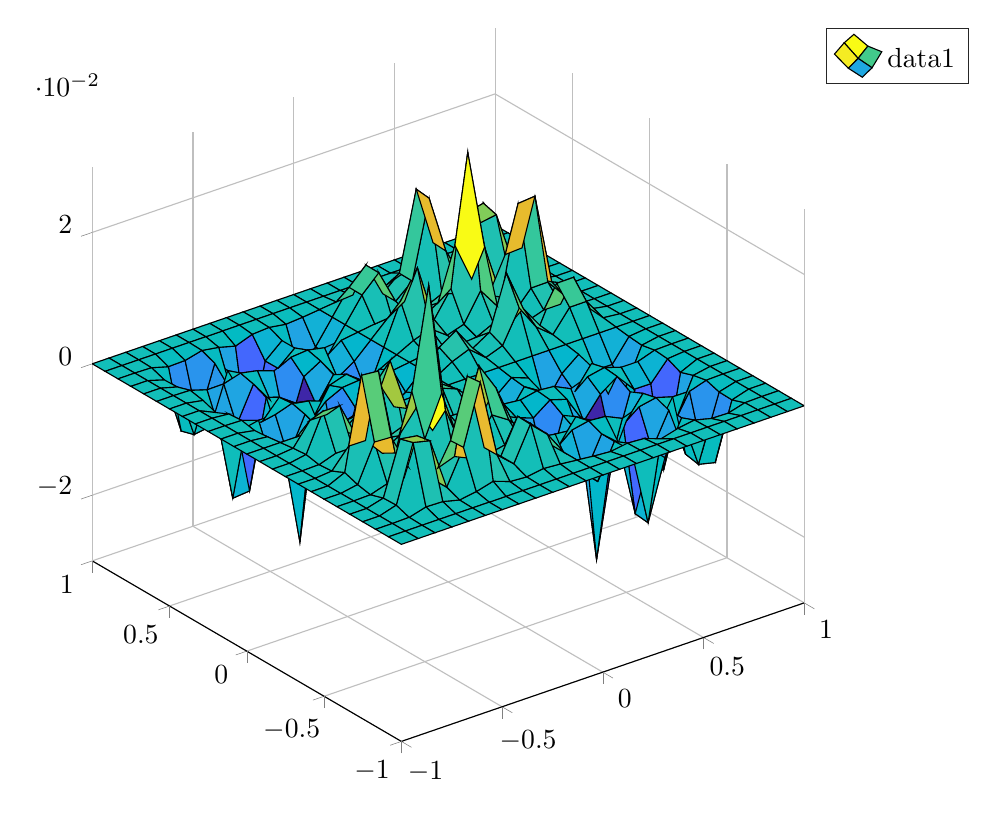
\begin{tikzpicture}

\begin{axis}[%
width=3.56in,
height=3.566in,
at={(0.597in,0.481in)},
scale only axis,
xmin=-1,
xmax=1,
tick align=outside,
ymin=-1,
ymax=1,
zmin=-0.03,
zmax=0.03,
view={-37.5}{30},
axis background/.style={fill=white},
axis x line*=bottom,
axis y line*=left,
axis z line*=left,
xmajorgrids,
ymajorgrids,
zmajorgrids,
legend style={at={(1.03,1)}, anchor=north west, legend cell align=left, align=left, draw=white!15!black}
]

\addplot3[%
surf,
shader=flat corner, draw=black, z buffer=sort, colormap={mymap}{[1pt] rgb(0pt)=(0.2422,0.1504,0.6603); rgb(1pt)=(0.25039,0.164995,0.707614); rgb(2pt)=(0.257771,0.181781,0.751138); rgb(3pt)=(0.264729,0.197757,0.795214); rgb(4pt)=(0.270648,0.214676,0.836371); rgb(5pt)=(0.275114,0.234238,0.870986); rgb(6pt)=(0.2783,0.255871,0.899071); rgb(7pt)=(0.280333,0.278233,0.9221); rgb(8pt)=(0.281338,0.300595,0.941376); rgb(9pt)=(0.281014,0.322757,0.957886); rgb(10pt)=(0.279467,0.344671,0.971676); rgb(11pt)=(0.275971,0.366681,0.982905); rgb(12pt)=(0.269914,0.3892,0.9906); rgb(13pt)=(0.260243,0.412329,0.995157); rgb(14pt)=(0.244033,0.435833,0.998833); rgb(15pt)=(0.220643,0.460257,0.997286); rgb(16pt)=(0.196333,0.484719,0.989152); rgb(17pt)=(0.183405,0.507371,0.979795); rgb(18pt)=(0.178643,0.528857,0.968157); rgb(19pt)=(0.176438,0.549905,0.952019); rgb(20pt)=(0.168743,0.570262,0.935871); rgb(21pt)=(0.154,0.5902,0.9218); rgb(22pt)=(0.146029,0.609119,0.907857); rgb(23pt)=(0.138024,0.627629,0.89729); rgb(24pt)=(0.124814,0.645929,0.888343); rgb(25pt)=(0.111252,0.6635,0.876314); rgb(26pt)=(0.0952095,0.679829,0.859781); rgb(27pt)=(0.0688714,0.694771,0.839357); rgb(28pt)=(0.0296667,0.708167,0.816333); rgb(29pt)=(0.00357143,0.720267,0.7917); rgb(30pt)=(0.00665714,0.731214,0.766014); rgb(31pt)=(0.0433286,0.741095,0.73941); rgb(32pt)=(0.0963952,0.75,0.712038); rgb(33pt)=(0.140771,0.7584,0.684157); rgb(34pt)=(0.1717,0.766962,0.655443); rgb(35pt)=(0.193767,0.775767,0.6251); rgb(36pt)=(0.216086,0.7843,0.5923); rgb(37pt)=(0.246957,0.791795,0.556743); rgb(38pt)=(0.290614,0.79729,0.518829); rgb(39pt)=(0.340643,0.8008,0.478857); rgb(40pt)=(0.3909,0.802871,0.435448); rgb(41pt)=(0.445629,0.802419,0.390919); rgb(42pt)=(0.5044,0.7993,0.348); rgb(43pt)=(0.561562,0.794233,0.304481); rgb(44pt)=(0.617395,0.787619,0.261238); rgb(45pt)=(0.671986,0.779271,0.2227); rgb(46pt)=(0.7242,0.769843,0.191029); rgb(47pt)=(0.773833,0.759805,0.16461); rgb(48pt)=(0.820314,0.749814,0.153529); rgb(49pt)=(0.863433,0.7406,0.159633); rgb(50pt)=(0.903543,0.733029,0.177414); rgb(51pt)=(0.939257,0.728786,0.209957); rgb(52pt)=(0.972757,0.729771,0.239443); rgb(53pt)=(0.995648,0.743371,0.237148); rgb(54pt)=(0.996986,0.765857,0.219943); rgb(55pt)=(0.995205,0.789252,0.202762); rgb(56pt)=(0.9892,0.813567,0.188533); rgb(57pt)=(0.978629,0.838629,0.176557); rgb(58pt)=(0.967648,0.8639,0.16429); rgb(59pt)=(0.96101,0.889019,0.153676); rgb(60pt)=(0.959671,0.913457,0.142257); rgb(61pt)=(0.962795,0.937338,0.12651); rgb(62pt)=(0.969114,0.960629,0.106362); rgb(63pt)=(0.9769,0.9839,0.0805)}, mesh/rows=25]
table[row sep=crcr, point meta=\thisrow{c}] {%
%
x	y	z	c\\
-1	-1	0	0\\
-0.916666666666667	-1	0	0\\
-0.833333333333333	-1	1.02695723625141e-24	1.02695723625141e-24\\
-0.75	-1	0	0\\
-0.666666666666667	-1	0	0\\
-0.583333333333333	-1	0	0\\
-0.5	-1	0	0\\
-0.416666666666667	-1	0	0\\
-0.333333333333333	-1	0	0\\
-0.25	-1	0	0\\
-0.166666666666667	-1	0	0\\
-0.0833333333333334	-1	0	0\\
0	-1	0	0\\
0.0833333333333333	-1	0	0\\
0.166666666666667	-1	0	0\\
0.25	-1	0	0\\
0.333333333333333	-1	0	0\\
0.416666666666667	-1	0	0\\
0.5	-1	0	0\\
0.583333333333333	-1	0	0\\
0.666666666666667	-1	0	0\\
0.75	-1	0	0\\
0.833333333333333	-1	0	0\\
0.916666666666667	-1	-4.38399307163469e-27	-4.38399307163469e-27\\
1	-1	0	0\\
-1	-0.916666666666667	0	0\\
-0.916666666666667	-0.916666666666667	2.55753406345044e-09	2.55753406345044e-09\\
-0.833333333333333	-0.916666666666667	3.85777718973534e-07	3.85777718973534e-07\\
-0.75	-0.916666666666667	4.17100875631788e-06	4.17100875631788e-06\\
-0.666666666666667	-0.916666666666667	3.64929550800072e-06	3.64929550800072e-06\\
-0.583333333333333	-0.916666666666667	3.45860111752149e-07	3.45860111752149e-07\\
-0.5	-0.916666666666667	2.33954300020683e-06	2.33954300020683e-06\\
-0.416666666666667	-0.916666666666667	5.70854139583692e-06	5.70854139583692e-06\\
-0.333333333333333	-0.916666666666667	1.17920908563584e-06	1.17920908563584e-06\\
-0.25	-0.916666666666667	3.45029265806706e-07	3.45029265806706e-07\\
-0.166666666666667	-0.916666666666667	2.26755661545572e-06	2.26755661545572e-06\\
-0.0833333333333334	-0.916666666666667	1.33785564740444e-06	1.33785564740444e-06\\
0	-0.916666666666667	-4.2425755489483e-22	-4.2425755489483e-22\\
0.0833333333333333	-0.916666666666667	-1.33785564740444e-06	-1.33785564740444e-06\\
0.166666666666667	-0.916666666666667	-2.26755661545571e-06	-2.26755661545571e-06\\
0.25	-0.916666666666667	-3.45029265806705e-07	-3.45029265806705e-07\\
0.333333333333333	-0.916666666666667	-1.17920908563584e-06	-1.17920908563584e-06\\
0.416666666666667	-0.916666666666667	-5.70854139583693e-06	-5.70854139583693e-06\\
0.5	-0.916666666666667	-2.33954300020683e-06	-2.33954300020683e-06\\
0.583333333333333	-0.916666666666667	-3.4586011175215e-07	-3.4586011175215e-07\\
0.666666666666667	-0.916666666666667	-3.64929550800072e-06	-3.64929550800072e-06\\
0.75	-0.916666666666667	-4.17100875631788e-06	-4.17100875631788e-06\\
0.833333333333333	-0.916666666666667	-3.85777718973533e-07	-3.85777718973533e-07\\
0.916666666666667	-0.916666666666667	-2.55753406345042e-09	-2.55753406345042e-09\\
1	-0.916666666666667	0	0\\
-1	-0.833333333333333	1.02695723625141e-24	1.02695723625141e-24\\
-0.916666666666667	-0.833333333333333	3.85777718973533e-07	3.85777718973533e-07\\
-0.833333333333333	-0.833333333333333	6.71198962422951e-05	6.71198962422951e-05\\
-0.75	-0.833333333333333	0.000778127800887982	0.000778127800887982\\
-0.666666666666667	-0.833333333333333	0.000707315736756557	0.000707315736756557\\
-0.583333333333333	-0.833333333333333	6.86074746915453e-05	6.86074746915453e-05\\
-0.5	-0.833333333333333	0.000471138162446881	0.000471138162446881\\
-0.416666666666667	-0.833333333333333	0.00116140316014542	0.00116140316014542\\
-0.333333333333333	-0.833333333333333	0.000241610914204461	0.000241610914204461\\
-0.25	-0.833333333333333	7.10368896279139e-05	7.10368896279139e-05\\
-0.166666666666667	-0.833333333333333	0.000468336406285743	0.000468336406285743\\
-0.0833333333333334	-0.833333333333333	0.000276812375771035	0.000276812375771035\\
0	-0.833333333333333	-7.74552301490904e-20	-7.74552301490904e-20\\
0.0833333333333333	-0.833333333333333	-0.000276812375771035	-0.000276812375771035\\
0.166666666666667	-0.833333333333333	-0.000468336406285742	-0.000468336406285742\\
0.25	-0.833333333333333	-7.10368896279136e-05	-7.10368896279136e-05\\
0.333333333333333	-0.833333333333333	-0.00024161091420446	-0.00024161091420446\\
0.416666666666667	-0.833333333333333	-0.00116140316014542	-0.00116140316014542\\
0.5	-0.833333333333333	-0.000471138162446881	-0.000471138162446881\\
0.583333333333333	-0.833333333333333	-6.86074746915456e-05	-6.86074746915456e-05\\
0.666666666666667	-0.833333333333333	-0.000707315736756559	-0.000707315736756559\\
0.75	-0.833333333333333	-0.000778127800887981	-0.000778127800887981\\
0.833333333333333	-0.833333333333333	-6.7119896242295e-05	-6.7119896242295e-05\\
0.916666666666667	-0.833333333333333	-3.85777718973525e-07	-3.85777718973525e-07\\
1	-0.833333333333333	-1.0269572362514e-24	-1.0269572362514e-24\\
-1	-0.75	0	0\\
-0.916666666666667	-0.75	4.17100875631788e-06	4.17100875631788e-06\\
-0.833333333333333	-0.75	0.000778127800887983	0.000778127800887983\\
-0.75	-0.75	0.00943571698715445	0.00943571698715445\\
-0.666666666666667	-0.75	0.00882480124123988	0.00882480124123988\\
-0.583333333333333	-0.75	0.000872104526134152	0.000872104526134152\\
-0.5	-0.75	0.0060652983794619	0.0060652983794619\\
-0.416666666666667	-0.75	0.0150841772008774	0.0150841772008774\\
-0.333333333333333	-0.75	0.00315753528677166	0.00315753528677166\\
-0.25	-0.75	0.000932352964394895	0.000932352964394895\\
-0.166666666666667	-0.75	0.00616423466770155	0.00616423466770155\\
-0.0833333333333334	-0.75	0.00364924259814257	0.00364924259814257\\
0	-0.75	-8.76737641779841e-19	-8.76737641779841e-19\\
0.0833333333333333	-0.75	-0.00364924259814257	-0.00364924259814257\\
0.166666666666667	-0.75	-0.00616423466770154	-0.00616423466770154\\
0.25	-0.75	-0.000932352964394891	-0.000932352964394891\\
0.333333333333333	-0.75	-0.00315753528677164	-0.00315753528677164\\
0.416666666666667	-0.75	-0.0150841772008774	-0.0150841772008774\\
0.5	-0.75	-0.0060652983794619	-0.0060652983794619\\
0.583333333333333	-0.75	-0.000872104526134156	-0.000872104526134156\\
0.666666666666667	-0.75	-0.00882480124123989	-0.00882480124123989\\
0.75	-0.75	-0.00943571698715444	-0.00943571698715444\\
0.833333333333333	-0.75	-0.000778127800887982	-0.000778127800887982\\
0.916666666666667	-0.75	-4.17100875631781e-06	-4.17100875631781e-06\\
1	-0.75	0	0\\
-1	-0.666666666666667	0	0\\
-0.916666666666667	-0.666666666666667	3.64929550800072e-06	3.64929550800072e-06\\
-0.833333333333333	-0.666666666666667	0.000707315736756557	0.000707315736756557\\
-0.75	-0.666666666666667	0.00882480124123988	0.00882480124123988\\
-0.666666666666667	-0.666666666666667	0.00842066215543398	0.00842066215543398\\
-0.583333333333333	-0.666666666666667	0.000843966898384536	0.000843966898384536\\
-0.5	-0.666666666666667	0.00592857826938018	0.00592857826938018\\
-0.416666666666667	-0.666666666666667	0.0148502404760497	0.0148502404760497\\
-0.333333333333333	-0.666666666666667	0.00312456184123599	0.00312456184123599\\
-0.25	-0.666666666666667	0.000925942478032866	0.000925942478032866\\
-0.166666666666667	-0.666666666666667	0.00613646636398126	0.00613646636398126\\
-0.0833333333333334	-0.666666666666667	0.00363775449063844	0.00363775449063844\\
0	-0.666666666666667	-8.44331861748012e-19	-8.44331861748012e-19\\
0.0833333333333333	-0.666666666666667	-0.00363775449063844	-0.00363775449063844\\
0.166666666666667	-0.666666666666667	-0.00613646636398124	-0.00613646636398124\\
0.25	-0.666666666666667	-0.000925942478032862	-0.000925942478032862\\
0.333333333333333	-0.666666666666667	-0.00312456184123597	-0.00312456184123597\\
0.416666666666667	-0.666666666666667	-0.0148502404760497	-0.0148502404760497\\
0.5	-0.666666666666667	-0.00592857826938018	-0.00592857826938018\\
0.583333333333333	-0.666666666666667	-0.00084396689838454	-0.00084396689838454\\
0.666666666666667	-0.666666666666667	-0.00842066215543399	-0.00842066215543399\\
0.75	-0.666666666666667	-0.00882480124123987	-0.00882480124123987\\
0.833333333333333	-0.666666666666667	-0.000707315736756558	-0.000707315736756558\\
0.916666666666667	-0.666666666666667	-3.64929550800066e-06	-3.64929550800066e-06\\
1	-0.666666666666667	0	0\\
-1	-0.583333333333333	0	0\\
-0.916666666666667	-0.583333333333333	3.45860111752149e-07	3.45860111752149e-07\\
-0.833333333333333	-0.583333333333333	6.86074746915453e-05	6.86074746915453e-05\\
-0.75	-0.583333333333333	0.000872104526134152	0.000872104526134152\\
-0.666666666666667	-0.583333333333333	0.000843966898384536	0.000843966898384536\\
-0.583333333333333	-0.583333333333333	8.50681297213606e-05	8.50681297213606e-05\\
-0.5	-0.583333333333333	0.000592761470027727	0.000592761470027727\\
-0.416666666666667	-0.583333333333333	0.00149315597727987	0.00149315597727987\\
-0.333333333333333	-0.583333333333333	0.000315453871556334	0.000315453871556334\\
-0.25	-0.583333333333333	9.31814902686496e-05	9.31814902686496e-05\\
-0.166666666666667	-0.583333333333333	0.000618502248354859	0.000618502248354859\\
-0.0833333333333334	-0.583333333333333	0.000367064223668659	0.000367064223668659\\
0	-0.583333333333333	-7.40930762219607e-20	-7.40930762219607e-20\\
0.0833333333333333	-0.583333333333333	-0.000367064223668659	-0.000367064223668659\\
0.166666666666667	-0.583333333333333	-0.000618502248354857	-0.000618502248354857\\
0.25	-0.583333333333333	-9.31814902686491e-05	-9.31814902686491e-05\\
0.333333333333333	-0.583333333333333	-0.000315453871556332	-0.000315453871556332\\
0.416666666666667	-0.583333333333333	-0.00149315597727987	-0.00149315597727987\\
0.5	-0.583333333333333	-0.000592761470027727	-0.000592761470027727\\
0.583333333333333	-0.583333333333333	-8.50681297213611e-05	-8.50681297213611e-05\\
0.666666666666667	-0.583333333333333	-0.000843966898384538	-0.000843966898384538\\
0.75	-0.583333333333333	-0.00087210452613415	-0.00087210452613415\\
0.833333333333333	-0.583333333333333	-6.86074746915454e-05	-6.86074746915454e-05\\
0.916666666666667	-0.583333333333333	-3.45860111752143e-07	-3.45860111752143e-07\\
1	-0.583333333333333	0	0\\
-1	-0.5	0	0\\
-0.916666666666667	-0.5	2.33954300020683e-06	2.33954300020683e-06\\
-0.833333333333333	-0.5	0.000471138162446881	0.000471138162446881\\
-0.75	-0.5	0.0060652983794619	0.0060652983794619\\
-0.666666666666667	-0.5	0.00592857826938018	0.00592857826938018\\
-0.583333333333333	-0.5	0.000592761470027727	0.000592761470027727\\
-0.5	-0.5	0.00393294666281547	0.00393294666281547\\
-0.416666666666667	-0.5	0.00994977833558941	0.00994977833558941\\
-0.333333333333333	-0.5	0.00210867680461956	0.00210867680461956\\
-0.25	-0.5	0.000610455051438689	0.000610455051438689\\
-0.166666666666667	-0.5	0.00405241439845992	0.00405241439845992\\
-0.0833333333333334	-0.5	0.0024071556172955	0.0024071556172955\\
0	-0.5	-5.91805759022251e-19	-5.91805759022251e-19\\
0.0833333333333333	-0.5	-0.0024071556172955	-0.0024071556172955\\
0.166666666666667	-0.5	-0.00405241439845991	-0.00405241439845991\\
0.25	-0.5	-0.000610455051438686	-0.000610455051438686\\
0.333333333333333	-0.5	-0.00210867680461956	-0.00210867680461956\\
0.416666666666667	-0.5	-0.00994977833558942	-0.00994977833558942\\
0.5	-0.5	-0.00393294666281547	-0.00393294666281547\\
0.583333333333333	-0.5	-0.000592761470027729	-0.000592761470027729\\
0.666666666666667	-0.5	-0.00592857826938019	-0.00592857826938019\\
0.75	-0.5	-0.00606529837946189	-0.00606529837946189\\
0.833333333333333	-0.5	-0.000471138162446881	-0.000471138162446881\\
0.916666666666667	-0.5	-2.33954300020679e-06	-2.33954300020679e-06\\
1	-0.5	0	0\\
-1	-0.416666666666667	0	0\\
-0.916666666666667	-0.416666666666667	5.70854139583692e-06	5.70854139583692e-06\\
-0.833333333333333	-0.416666666666667	0.00116140316014542	0.00116140316014542\\
-0.75	-0.416666666666667	0.0150841772008774	0.0150841772008774\\
-0.666666666666667	-0.416666666666667	0.0148502404760497	0.0148502404760497\\
-0.583333333333333	-0.416666666666667	0.00149315597727987	0.00149315597727987\\
-0.5	-0.416666666666667	0.00994977833558941	0.00994977833558941\\
-0.416666666666667	-0.416666666666667	0.0252552578198303	0.0252552578198303\\
-0.333333333333333	-0.416666666666667	0.00536572588063085	0.00536572588063085\\
-0.25	-0.416666666666667	0.00155612453270233	0.00155612453270233\\
-0.166666666666667	-0.416666666666667	0.010342674976464	0.010342674976464\\
-0.0833333333333334	-0.416666666666667	0.00614793627719881	0.00614793627719881\\
0	-0.416666666666667	-1.50433859765667e-18	-1.50433859765667e-18\\
0.0833333333333333	-0.416666666666667	-0.0061479362771988	-0.0061479362771988\\
0.166666666666667	-0.416666666666667	-0.010342674976464	-0.010342674976464\\
0.25	-0.416666666666667	-0.00155612453270232	-0.00155612453270232\\
0.333333333333333	-0.416666666666667	-0.00536572588063083	-0.00536572588063083\\
0.416666666666667	-0.416666666666667	-0.0252552578198304	-0.0252552578198304\\
0.5	-0.416666666666667	-0.00994977833558941	-0.00994977833558941\\
0.583333333333333	-0.416666666666667	-0.00149315597727988	-0.00149315597727988\\
0.666666666666667	-0.416666666666667	-0.0148502404760497	-0.0148502404760497\\
0.75	-0.416666666666667	-0.0150841772008774	-0.0150841772008774\\
0.833333333333333	-0.416666666666667	-0.00116140316014542	-0.00116140316014542\\
0.916666666666667	-0.416666666666667	-5.70854139583682e-06	-5.70854139583682e-06\\
1	-0.416666666666667	0	0\\
-1	-0.333333333333333	0	0\\
-0.916666666666667	-0.333333333333333	1.17920908563584e-06	1.17920908563584e-06\\
-0.833333333333333	-0.333333333333333	0.000241610914204461	0.000241610914204461\\
-0.75	-0.333333333333333	0.00315753528677166	0.00315753528677166\\
-0.666666666666667	-0.333333333333333	0.00312456184123599	0.00312456184123599\\
-0.583333333333333	-0.333333333333333	0.000315453871556334	0.000315453871556334\\
-0.5	-0.333333333333333	0.00210867680461956	0.00210867680461956\\
-0.416666666666667	-0.333333333333333	0.00536572588063085	0.00536572588063085\\
-0.333333333333333	-0.333333333333333	0.00114214387023767	0.00114214387023767\\
-0.25	-0.333333333333333	0.000331677317790113	0.000331677317790113\\
-0.166666666666667	-0.333333333333333	0.00220651736235955	0.00220651736235955\\
-0.0833333333333334	-0.333333333333333	0.00131231582712499	0.00131231582712499\\
0	-0.333333333333333	-3.16585135024486e-19	-3.16585135024486e-19\\
0.0833333333333333	-0.333333333333333	-0.00131231582712499	-0.00131231582712499\\
0.166666666666667	-0.333333333333333	-0.00220651736235954	-0.00220651736235954\\
0.25	-0.333333333333333	-0.000331677317790112	-0.000331677317790112\\
0.333333333333333	-0.333333333333333	-0.00114214387023766	-0.00114214387023766\\
0.416666666666667	-0.333333333333333	-0.00536572588063086	-0.00536572588063086\\
0.5	-0.333333333333333	-0.00210867680461956	-0.00210867680461956\\
0.583333333333333	-0.333333333333333	-0.000315453871556335	-0.000315453871556335\\
0.666666666666667	-0.333333333333333	-0.00312456184123599	-0.00312456184123599\\
0.75	-0.333333333333333	-0.00315753528677165	-0.00315753528677165\\
0.833333333333333	-0.333333333333333	-0.000241610914204461	-0.000241610914204461\\
0.916666666666667	-0.333333333333333	-1.17920908563582e-06	-1.17920908563582e-06\\
1	-0.333333333333333	0	0\\
-1	-0.25	0	0\\
-0.916666666666667	-0.25	3.45029265806706e-07	3.45029265806706e-07\\
-0.833333333333333	-0.25	7.1036889627914e-05	7.1036889627914e-05\\
-0.75	-0.25	0.000932352964394894	0.000932352964394894\\
-0.666666666666667	-0.25	0.000925942478032866	0.000925942478032866\\
-0.583333333333333	-0.25	9.31814902686495e-05	9.31814902686495e-05\\
-0.5	-0.25	0.000610455051438689	0.000610455051438689\\
-0.416666666666667	-0.25	0.00155612453270233	0.00155612453270233\\
-0.333333333333333	-0.25	0.000331677317790113	0.000331677317790113\\
-0.25	-0.25	9.54350634367825e-05	9.54350634367825e-05\\
-0.166666666666667	-0.25	0.000634901021554919	0.000634901021554919\\
-0.0833333333333334	-0.25	0.00037775454883306	0.00037775454883306\\
0	-0.25	-8.80499813311504e-20	-8.80499813311504e-20\\
0.0833333333333333	-0.25	-0.00037775454883306	-0.00037775454883306\\
0.166666666666667	-0.25	-0.000634901021554917	-0.000634901021554917\\
0.25	-0.25	-9.54350634367821e-05	-9.54350634367821e-05\\
0.333333333333333	-0.25	-0.000331677317790112	-0.000331677317790112\\
0.416666666666667	-0.25	-0.00155612453270233	-0.00155612453270233\\
0.5	-0.25	-0.000610455051438689	-0.000610455051438689\\
0.583333333333333	-0.25	-9.31814902686498e-05	-9.31814902686498e-05\\
0.666666666666667	-0.25	-0.000925942478032867	-0.000925942478032867\\
0.75	-0.25	-0.000932352964394893	-0.000932352964394893\\
0.833333333333333	-0.25	-7.1036889627914e-05	-7.1036889627914e-05\\
0.916666666666667	-0.25	-3.450292658067e-07	-3.450292658067e-07\\
1	-0.25	0	0\\
-1	-0.166666666666667	0	0\\
-0.916666666666667	-0.166666666666667	2.26755661545572e-06	2.26755661545572e-06\\
-0.833333333333333	-0.166666666666667	0.000468336406285743	0.000468336406285743\\
-0.75	-0.166666666666667	0.00616423466770155	0.00616423466770155\\
-0.666666666666667	-0.166666666666667	0.00613646636398126	0.00613646636398126\\
-0.583333333333333	-0.166666666666667	0.000618502248354858	0.000618502248354858\\
-0.5	-0.166666666666667	0.00405241439845992	0.00405241439845992\\
-0.416666666666667	-0.166666666666667	0.010342674976464	0.010342674976464\\
-0.333333333333333	-0.166666666666667	0.00220651736235955	0.00220651736235955\\
-0.25	-0.166666666666667	0.000634901021554919	0.000634901021554919\\
-0.166666666666667	-0.166666666666667	0.00422559650685534	0.00422559650685534\\
-0.0833333333333334	-0.166666666666667	0.00251483803933617	0.00251483803933617\\
0	-0.166666666666667	-6.34758211468699e-19	-6.34758211468699e-19\\
0.0833333333333333	-0.166666666666667	-0.00251483803933617	-0.00251483803933617\\
0.166666666666667	-0.166666666666667	-0.00422559650685533	-0.00422559650685533\\
0.25	-0.166666666666667	-0.000634901021554916	-0.000634901021554916\\
0.333333333333333	-0.166666666666667	-0.00220651736235954	-0.00220651736235954\\
0.416666666666667	-0.166666666666667	-0.010342674976464	-0.010342674976464\\
0.5	-0.166666666666667	-0.00405241439845992	-0.00405241439845992\\
0.583333333333333	-0.166666666666667	-0.000618502248354861	-0.000618502248354861\\
0.666666666666667	-0.166666666666667	-0.00613646636398127	-0.00613646636398127\\
0.75	-0.166666666666667	-0.00616423466770154	-0.00616423466770154\\
0.833333333333333	-0.166666666666667	-0.000468336406285743	-0.000468336406285743\\
0.916666666666667	-0.166666666666667	-2.26755661545568e-06	-2.26755661545568e-06\\
1	-0.166666666666667	0	0\\
-1	-0.0833333333333334	0	0\\
-0.916666666666667	-0.0833333333333334	1.33785564740444e-06	1.33785564740444e-06\\
-0.833333333333333	-0.0833333333333334	0.000276812375771035	0.000276812375771035\\
-0.75	-0.0833333333333334	0.00364924259814257	0.00364924259814257\\
-0.666666666666667	-0.0833333333333334	0.00363775449063844	0.00363775449063844\\
-0.583333333333333	-0.0833333333333334	0.000367064223668659	0.000367064223668659\\
-0.5	-0.0833333333333334	0.0024071556172955	0.0024071556172955\\
-0.416666666666667	-0.0833333333333334	0.0061479362771988	0.0061479362771988\\
-0.333333333333333	-0.0833333333333334	0.00131231582712499	0.00131231582712499\\
-0.25	-0.0833333333333334	0.00037775454883306	0.00037775454883306\\
-0.166666666666667	-0.0833333333333334	0.00251483803933617	0.00251483803933617\\
-0.0833333333333334	-0.0833333333333334	0.0014969284339611	0.0014969284339611\\
0	-0.0833333333333334	-4.12134423225633e-19	-4.12134423225633e-19\\
0.0833333333333333	-0.0833333333333334	-0.0014969284339611	-0.0014969284339611\\
0.166666666666667	-0.0833333333333334	-0.00251483803933616	-0.00251483803933616\\
0.25	-0.0833333333333334	-0.000377754548833058	-0.000377754548833058\\
0.333333333333333	-0.0833333333333334	-0.00131231582712498	-0.00131231582712498\\
0.416666666666667	-0.0833333333333334	-0.00614793627719881	-0.00614793627719881\\
0.5	-0.0833333333333334	-0.00240715561729551	-0.00240715561729551\\
0.583333333333333	-0.0833333333333334	-0.000367064223668661	-0.000367064223668661\\
0.666666666666667	-0.0833333333333334	-0.00363775449063844	-0.00363775449063844\\
0.75	-0.0833333333333334	-0.00364924259814256	-0.00364924259814256\\
0.833333333333333	-0.0833333333333334	-0.000276812375771035	-0.000276812375771035\\
0.916666666666667	-0.0833333333333334	-1.33785564740442e-06	-1.33785564740442e-06\\
1	-0.0833333333333334	0	0\\
-1	0	0	0\\
-0.916666666666667	0	-4.22019650749432e-22	-4.22019650749432e-22\\
-0.833333333333333	0	-7.58062703141482e-20	-7.58062703141482e-20\\
-0.75	0	-8.8948973557021e-19	-8.8948973557021e-19\\
-0.666666666666667	0	-8.48925864908015e-19	-8.48925864908015e-19\\
-0.583333333333333	0	-7.4663668535476e-20	-7.4663668535476e-20\\
-0.5	0	-6.59299545930563e-19	-6.59299545930563e-19\\
-0.416666666666667	0	-1.65655633099897e-18	-1.65655633099897e-18\\
-0.333333333333333	0	-3.57084812293917e-19	-3.57084812293917e-19\\
-0.25	0	-8.37743870326049e-20	-8.37743870326049e-20\\
-0.166666666666667	0	-6.03879200828298e-19	-6.03879200828298e-19\\
-0.0833333333333334	0	-3.932851103973e-19	-3.932851103973e-19\\
0	0	-4.82118586296267e-21	-4.82118586296267e-21\\
0.0833333333333333	0	4.48056541275829e-19	4.48056541275829e-19\\
0.166666666666667	0	6.75165917404855e-19	6.75165917404855e-19\\
0.25	0	8.05379513898792e-20	8.05379513898792e-20\\
0.333333333333333	0	3.00487456194101e-19	3.00487456194101e-19\\
0.416666666666667	0	1.62580333661468e-18	1.62580333661468e-18\\
0.5	0	5.57212921187685e-19	5.57212921187685e-19\\
0.583333333333333	0	9.80093456331336e-20	9.80093456331336e-20\\
0.666666666666667	0	8.61737011716055e-19	8.61737011716055e-19\\
0.75	0	9.60761298722394e-19	9.60761298722394e-19\\
0.833333333333333	0	7.99192795843061e-20	7.99192795843061e-20\\
0.916666666666667	0	3.15236993062634e-22	3.15236993062634e-22\\
1	0	0	0\\
-1	0.0833333333333333	0	0\\
-0.916666666666667	0.0833333333333333	-1.33785564740444e-06	-1.33785564740444e-06\\
-0.833333333333333	0.0833333333333333	-0.000276812375771035	-0.000276812375771035\\
-0.75	0.0833333333333333	-0.00364924259814257	-0.00364924259814257\\
-0.666666666666667	0.0833333333333333	-0.00363775449063844	-0.00363775449063844\\
-0.583333333333333	0.0833333333333333	-0.000367064223668659	-0.000367064223668659\\
-0.5	0.0833333333333333	-0.0024071556172955	-0.0024071556172955\\
-0.416666666666667	0.0833333333333333	-0.0061479362771988	-0.0061479362771988\\
-0.333333333333333	0.0833333333333333	-0.00131231582712499	-0.00131231582712499\\
-0.25	0.0833333333333333	-0.00037775454883306	-0.00037775454883306\\
-0.166666666666667	0.0833333333333333	-0.00251483803933617	-0.00251483803933617\\
-0.0833333333333334	0.0833333333333333	-0.0014969284339611	-0.0014969284339611\\
0	0.0833333333333333	4.51410925247731e-19	4.51410925247731e-19\\
0.0833333333333333	0.0833333333333333	0.0014969284339611	0.0014969284339611\\
0.166666666666667	0.0833333333333333	0.00251483803933616	0.00251483803933616\\
0.25	0.0833333333333333	0.000377754548833058	0.000377754548833058\\
0.333333333333333	0.0833333333333333	0.00131231582712498	0.00131231582712498\\
0.416666666666667	0.0833333333333333	0.00614793627719881	0.00614793627719881\\
0.5	0.0833333333333333	0.0024071556172955	0.0024071556172955\\
0.583333333333333	0.0833333333333333	0.00036706422366866	0.00036706422366866\\
0.666666666666667	0.0833333333333333	0.00363775449063844	0.00363775449063844\\
0.75	0.0833333333333333	0.00364924259814256	0.00364924259814256\\
0.833333333333333	0.0833333333333333	0.000276812375771035	0.000276812375771035\\
0.916666666666667	0.0833333333333333	1.33785564740442e-06	1.33785564740442e-06\\
1	0.0833333333333333	0	0\\
-1	0.166666666666667	0	0\\
-0.916666666666667	0.166666666666667	-2.26755661545571e-06	-2.26755661545571e-06\\
-0.833333333333333	0.166666666666667	-0.000468336406285741	-0.000468336406285741\\
-0.75	0.166666666666667	-0.00616423466770153	-0.00616423466770153\\
-0.666666666666667	0.166666666666667	-0.00613646636398124	-0.00613646636398124\\
-0.583333333333333	0.166666666666667	-0.000618502248354857	-0.000618502248354857\\
-0.5	0.166666666666667	-0.00405241439845991	-0.00405241439845991\\
-0.416666666666667	0.166666666666667	-0.010342674976464	-0.010342674976464\\
-0.333333333333333	0.166666666666667	-0.00220651736235954	-0.00220651736235954\\
-0.25	0.166666666666667	-0.000634901021554917	-0.000634901021554917\\
-0.166666666666667	0.166666666666667	-0.00422559650685533	-0.00422559650685533\\
-0.0833333333333334	0.166666666666667	-0.00251483803933616	-0.00251483803933616\\
0	0.166666666666667	6.9848421185914e-19	6.9848421185914e-19\\
0.0833333333333333	0.166666666666667	0.00251483803933616	0.00251483803933616\\
0.166666666666667	0.166666666666667	0.00422559650685532	0.00422559650685532\\
0.25	0.166666666666667	0.000634901021554914	0.000634901021554914\\
0.333333333333333	0.166666666666667	0.00220651736235953	0.00220651736235953\\
0.416666666666667	0.166666666666667	0.010342674976464	0.010342674976464\\
0.5	0.166666666666667	0.00405241439845991	0.00405241439845991\\
0.583333333333333	0.166666666666667	0.000618502248354859	0.000618502248354859\\
0.666666666666667	0.166666666666667	0.00613646636398125	0.00613646636398125\\
0.75	0.166666666666667	0.00616423466770152	0.00616423466770152\\
0.833333333333333	0.166666666666667	0.000468336406285741	0.000468336406285741\\
0.916666666666667	0.166666666666667	2.26755661545567e-06	2.26755661545567e-06\\
1	0.166666666666667	0	0\\
-1	0.25	0	0\\
-0.916666666666667	0.25	-3.45029265806704e-07	-3.45029265806704e-07\\
-0.833333333333333	0.25	-7.10368896279136e-05	-7.10368896279136e-05\\
-0.75	0.25	-0.000932352964394891	-0.000932352964394891\\
-0.666666666666667	0.25	-0.000925942478032862	-0.000925942478032862\\
-0.583333333333333	0.25	-9.31814902686491e-05	-9.31814902686491e-05\\
-0.5	0.25	-0.000610455051438686	-0.000610455051438686\\
-0.416666666666667	0.25	-0.00155612453270232	-0.00155612453270232\\
-0.333333333333333	0.25	-0.000331677317790112	-0.000331677317790112\\
-0.25	0.25	-9.5435063436782e-05	-9.5435063436782e-05\\
-0.166666666666667	0.25	-0.000634901021554916	-0.000634901021554916\\
-0.0833333333333334	0.25	-0.000377754548833058	-0.000377754548833058\\
0	0.25	7.94089675468141e-20	7.94089675468141e-20\\
0.0833333333333333	0.25	0.000377754548833058	0.000377754548833058\\
0.166666666666667	0.25	0.000634901021554914	0.000634901021554914\\
0.25	0.25	9.54350634367817e-05	9.54350634367817e-05\\
0.333333333333333	0.25	0.000331677317790111	0.000331677317790111\\
0.416666666666667	0.25	0.00155612453270232	0.00155612453270232\\
0.5	0.25	0.000610455051438686	0.000610455051438686\\
0.583333333333333	0.25	9.31814902686495e-05	9.31814902686495e-05\\
0.666666666666667	0.25	0.000925942478032864	0.000925942478032864\\
0.75	0.25	0.000932352964394889	0.000932352964394889\\
0.833333333333333	0.25	7.10368896279137e-05	7.10368896279137e-05\\
0.916666666666667	0.25	3.45029265806699e-07	3.45029265806699e-07\\
1	0.25	0	0\\
-1	0.333333333333333	0	0\\
-0.916666666666667	0.333333333333333	-1.17920908563583e-06	-1.17920908563583e-06\\
-0.833333333333333	0.333333333333333	-0.00024161091420446	-0.00024161091420446\\
-0.75	0.333333333333333	-0.00315753528677164	-0.00315753528677164\\
-0.666666666666667	0.333333333333333	-0.00312456184123597	-0.00312456184123597\\
-0.583333333333333	0.333333333333333	-0.000315453871556332	-0.000315453871556332\\
-0.5	0.333333333333333	-0.00210867680461956	-0.00210867680461956\\
-0.416666666666667	0.333333333333333	-0.00536572588063083	-0.00536572588063083\\
-0.333333333333333	0.333333333333333	-0.00114214387023766	-0.00114214387023766\\
-0.25	0.333333333333333	-0.000331677317790112	-0.000331677317790112\\
-0.166666666666667	0.333333333333333	-0.00220651736235954	-0.00220651736235954\\
-0.0833333333333334	0.333333333333333	-0.00131231582712498	-0.00131231582712498\\
0	0.333333333333333	3.22485562489602e-19	3.22485562489602e-19\\
0.0833333333333333	0.333333333333333	0.00131231582712498	0.00131231582712498\\
0.166666666666667	0.333333333333333	0.00220651736235953	0.00220651736235953\\
0.25	0.333333333333333	0.000331677317790111	0.000331677317790111\\
0.333333333333333	0.333333333333333	0.00114214387023766	0.00114214387023766\\
0.416666666666667	0.333333333333333	0.00536572588063084	0.00536572588063084\\
0.5	0.333333333333333	0.00210867680461956	0.00210867680461956\\
0.583333333333333	0.333333333333333	0.000315453871556334	0.000315453871556334\\
0.666666666666667	0.333333333333333	0.00312456184123598	0.00312456184123598\\
0.75	0.333333333333333	0.00315753528677164	0.00315753528677164\\
0.833333333333333	0.333333333333333	0.00024161091420446	0.00024161091420446\\
0.916666666666667	0.333333333333333	1.17920908563582e-06	1.17920908563582e-06\\
1	0.333333333333333	0	0\\
-1	0.416666666666667	0	0\\
-0.916666666666667	0.416666666666667	-5.70854139583693e-06	-5.70854139583693e-06\\
-0.833333333333333	0.416666666666667	-0.00116140316014542	-0.00116140316014542\\
-0.75	0.416666666666667	-0.0150841772008774	-0.0150841772008774\\
-0.666666666666667	0.416666666666667	-0.0148502404760497	-0.0148502404760497\\
-0.583333333333333	0.416666666666667	-0.00149315597727987	-0.00149315597727987\\
-0.5	0.416666666666667	-0.00994977833558942	-0.00994977833558942\\
-0.416666666666667	0.416666666666667	-0.0252552578198304	-0.0252552578198304\\
-0.333333333333333	0.416666666666667	-0.00536572588063086	-0.00536572588063086\\
-0.25	0.416666666666667	-0.00155612453270233	-0.00155612453270233\\
-0.166666666666667	0.416666666666667	-0.010342674976464	-0.010342674976464\\
-0.0833333333333334	0.416666666666667	-0.00614793627719881	-0.00614793627719881\\
0	0.416666666666667	1.70743447471519e-18	1.70743447471519e-18\\
0.0833333333333333	0.416666666666667	0.00614793627719881	0.00614793627719881\\
0.166666666666667	0.416666666666667	0.010342674976464	0.010342674976464\\
0.25	0.416666666666667	0.00155612453270232	0.00155612453270232\\
0.333333333333333	0.416666666666667	0.00536572588063084	0.00536572588063084\\
0.416666666666667	0.416666666666667	0.0252552578198304	0.0252552578198304\\
0.5	0.416666666666667	0.00994977833558942	0.00994977833558942\\
0.583333333333333	0.416666666666667	0.00149315597727988	0.00149315597727988\\
0.666666666666667	0.416666666666667	0.0148502404760497	0.0148502404760497\\
0.75	0.416666666666667	0.0150841772008774	0.0150841772008774\\
0.833333333333333	0.416666666666667	0.00116140316014542	0.00116140316014542\\
0.916666666666667	0.416666666666667	5.70854139583684e-06	5.70854139583684e-06\\
1	0.416666666666667	0	0\\
-1	0.5	0	0\\
-0.916666666666667	0.5	-2.33954300020683e-06	-2.33954300020683e-06\\
-0.833333333333333	0.5	-0.000471138162446881	-0.000471138162446881\\
-0.75	0.5	-0.0060652983794619	-0.0060652983794619\\
-0.666666666666667	0.5	-0.00592857826938018	-0.00592857826938018\\
-0.583333333333333	0.5	-0.000592761470027727	-0.000592761470027727\\
-0.5	0.5	-0.00393294666281547	-0.00393294666281547\\
-0.416666666666667	0.5	-0.00994977833558941	-0.00994977833558941\\
-0.333333333333333	0.5	-0.00210867680461956	-0.00210867680461956\\
-0.25	0.5	-0.000610455051438689	-0.000610455051438689\\
-0.166666666666667	0.5	-0.00405241439845992	-0.00405241439845992\\
-0.0833333333333334	0.5	-0.00240715561729551	-0.00240715561729551\\
0	0.5	5.92452022970232e-19	5.92452022970232e-19\\
0.0833333333333333	0.5	0.0024071556172955	0.0024071556172955\\
0.166666666666667	0.5	0.00405241439845991	0.00405241439845991\\
0.25	0.5	0.000610455051438686	0.000610455051438686\\
0.333333333333333	0.5	0.00210867680461956	0.00210867680461956\\
0.416666666666667	0.5	0.00994977833558942	0.00994977833558942\\
0.5	0.5	0.00393294666281547	0.00393294666281547\\
0.583333333333333	0.5	0.000592761470027729	0.000592761470027729\\
0.666666666666667	0.5	0.00592857826938019	0.00592857826938019\\
0.75	0.5	0.00606529837946189	0.00606529837946189\\
0.833333333333333	0.5	0.000471138162446881	0.000471138162446881\\
0.916666666666667	0.5	2.33954300020679e-06	2.33954300020679e-06\\
1	0.5	0	0\\
-1	0.583333333333333	0	0\\
-0.916666666666667	0.583333333333333	-3.45860111752151e-07	-3.45860111752151e-07\\
-0.833333333333333	0.583333333333333	-6.86074746915456e-05	-6.86074746915456e-05\\
-0.75	0.583333333333333	-0.000872104526134156	-0.000872104526134156\\
-0.666666666666667	0.583333333333333	-0.00084396689838454	-0.00084396689838454\\
-0.583333333333333	0.583333333333333	-8.50681297213611e-05	-8.50681297213611e-05\\
-0.5	0.583333333333333	-0.000592761470027729	-0.000592761470027729\\
-0.416666666666667	0.583333333333333	-0.00149315597727988	-0.00149315597727988\\
-0.333333333333333	0.583333333333333	-0.000315453871556335	-0.000315453871556335\\
-0.25	0.583333333333333	-9.31814902686498e-05	-9.31814902686498e-05\\
-0.166666666666667	0.583333333333333	-0.000618502248354861	-0.000618502248354861\\
-0.0833333333333334	0.583333333333333	-0.000367064223668661	-0.000367064223668661\\
0	0.583333333333333	1.04971725804411e-19	1.04971725804411e-19\\
0.0833333333333333	0.583333333333333	0.00036706422366866	0.00036706422366866\\
0.166666666666667	0.583333333333333	0.00061850224835486	0.00061850224835486\\
0.25	0.583333333333333	9.31814902686495e-05	9.31814902686495e-05\\
0.333333333333333	0.583333333333333	0.000315453871556334	0.000315453871556334\\
0.416666666666667	0.583333333333333	0.00149315597727988	0.00149315597727988\\
0.5	0.583333333333333	0.000592761470027729	0.000592761470027729\\
0.583333333333333	0.583333333333333	8.50681297213614e-05	8.50681297213614e-05\\
0.666666666666667	0.583333333333333	0.000843966898384542	0.000843966898384542\\
0.75	0.583333333333333	0.000872104526134154	0.000872104526134154\\
0.833333333333333	0.583333333333333	6.86074746915456e-05	6.86074746915456e-05\\
0.916666666666667	0.583333333333333	3.45860111752145e-07	3.45860111752145e-07\\
1	0.583333333333333	0	0\\
-1	0.666666666666667	0	0\\
-0.916666666666667	0.666666666666667	-3.64929550800073e-06	-3.64929550800073e-06\\
-0.833333333333333	0.666666666666667	-0.00070731573675656	-0.00070731573675656\\
-0.75	0.666666666666667	-0.0088248012412399	-0.0088248012412399\\
-0.666666666666667	0.666666666666667	-0.008420662155434	-0.008420662155434\\
-0.583333333333333	0.666666666666667	-0.000843966898384539	-0.000843966898384539\\
-0.5	0.666666666666667	-0.00592857826938019	-0.00592857826938019\\
-0.416666666666667	0.666666666666667	-0.0148502404760497	-0.0148502404760497\\
-0.333333333333333	0.666666666666667	-0.00312456184123599	-0.00312456184123599\\
-0.25	0.666666666666667	-0.000925942478032867	-0.000925942478032867\\
-0.166666666666667	0.666666666666667	-0.00613646636398127	-0.00613646636398127\\
-0.0833333333333334	0.666666666666667	-0.00363775449063844	-0.00363775449063844\\
0	0.666666666666667	9.33310259723488e-19	9.33310259723488e-19\\
0.0833333333333333	0.666666666666667	0.00363775449063844	0.00363775449063844\\
0.166666666666667	0.666666666666667	0.00613646636398125	0.00613646636398125\\
0.25	0.666666666666667	0.000925942478032864	0.000925942478032864\\
0.333333333333333	0.666666666666667	0.00312456184123598	0.00312456184123598\\
0.416666666666667	0.666666666666667	0.0148502404760497	0.0148502404760497\\
0.5	0.666666666666667	0.00592857826938019	0.00592857826938019\\
0.583333333333333	0.666666666666667	0.000843966898384542	0.000843966898384542\\
0.666666666666667	0.666666666666667	0.00842066215543401	0.00842066215543401\\
0.75	0.666666666666667	0.00882480124123988	0.00882480124123988\\
0.833333333333333	0.666666666666667	0.00070731573675656	0.00070731573675656\\
0.916666666666667	0.666666666666667	3.64929550800067e-06	3.64929550800067e-06\\
1	0.666666666666667	0	0\\
-1	0.75	0	0\\
-0.916666666666667	0.75	-4.17100875631788e-06	-4.17100875631788e-06\\
-0.833333333333333	0.75	-0.000778127800887982	-0.000778127800887982\\
-0.75	0.75	-0.00943571698715445	-0.00943571698715445\\
-0.666666666666667	0.75	-0.00882480124123987	-0.00882480124123987\\
-0.583333333333333	0.75	-0.000872104526134151	-0.000872104526134151\\
-0.5	0.75	-0.00606529837946189	-0.00606529837946189\\
-0.416666666666667	0.75	-0.0150841772008774	-0.0150841772008774\\
-0.333333333333333	0.75	-0.00315753528677165	-0.00315753528677165\\
-0.25	0.75	-0.000932352964394893	-0.000932352964394893\\
-0.166666666666667	0.75	-0.00616423466770154	-0.00616423466770154\\
-0.0833333333333334	0.75	-0.00364924259814256	-0.00364924259814256\\
0	0.75	1.06575368959258e-18	1.06575368959258e-18\\
0.0833333333333333	0.75	0.00364924259814256	0.00364924259814256\\
0.166666666666667	0.75	0.00616423466770153	0.00616423466770153\\
0.25	0.75	0.00093235296439489	0.00093235296439489\\
0.333333333333333	0.75	0.00315753528677164	0.00315753528677164\\
0.416666666666667	0.75	0.0150841772008774	0.0150841772008774\\
0.5	0.75	0.00606529837946189	0.00606529837946189\\
0.583333333333333	0.75	0.000872104526134154	0.000872104526134154\\
0.666666666666667	0.75	0.00882480124123988	0.00882480124123988\\
0.75	0.75	0.00943571698715443	0.00943571698715443\\
0.833333333333333	0.75	0.000778127800887981	0.000778127800887981\\
0.916666666666667	0.75	4.17100875631781e-06	4.17100875631781e-06\\
1	0.75	0	0\\
-1	0.833333333333333	0	0\\
-0.916666666666667	0.833333333333333	-3.85777718973533e-07	-3.85777718973533e-07\\
-0.833333333333333	0.833333333333333	-6.71198962422952e-05	-6.71198962422952e-05\\
-0.75	0.833333333333333	-0.000778127800887983	-0.000778127800887983\\
-0.666666666666667	0.833333333333333	-0.00070731573675656	-0.00070731573675656\\
-0.583333333333333	0.833333333333333	-6.86074746915454e-05	-6.86074746915454e-05\\
-0.5	0.833333333333333	-0.000471138162446881	-0.000471138162446881\\
-0.416666666666667	0.833333333333333	-0.00116140316014542	-0.00116140316014542\\
-0.333333333333333	0.833333333333333	-0.000241610914204461	-0.000241610914204461\\
-0.25	0.833333333333333	-7.1036889627914e-05	-7.1036889627914e-05\\
-0.166666666666667	0.833333333333333	-0.000468336406285743	-0.000468336406285743\\
-0.0833333333333334	0.833333333333333	-0.000276812375771035	-0.000276812375771035\\
0	0.833333333333333	8.37694525397532e-20	8.37694525397532e-20\\
0.0833333333333333	0.833333333333333	0.000276812375771035	0.000276812375771035\\
0.166666666666667	0.833333333333333	0.000468336406285742	0.000468336406285742\\
0.25	0.833333333333333	7.10368896279137e-05	7.10368896279137e-05\\
0.333333333333333	0.833333333333333	0.00024161091420446	0.00024161091420446\\
0.416666666666667	0.833333333333333	0.00116140316014542	0.00116140316014542\\
0.5	0.833333333333333	0.000471138162446881	0.000471138162446881\\
0.583333333333333	0.833333333333333	6.86074746915456e-05	6.86074746915456e-05\\
0.666666666666667	0.833333333333333	0.000707315736756561	0.000707315736756561\\
0.75	0.833333333333333	0.000778127800887981	0.000778127800887981\\
0.833333333333333	0.833333333333333	6.71198962422952e-05	6.71198962422952e-05\\
0.916666666666667	0.833333333333333	3.85777718973525e-07	3.85777718973525e-07\\
1	0.833333333333333	0	0\\
-1	0.916666666666667	-4.38399307163469e-27	-4.38399307163469e-27\\
-0.916666666666667	0.916666666666667	-2.55753406345044e-09	-2.55753406345044e-09\\
-0.833333333333333	0.916666666666667	-3.85777718973526e-07	-3.85777718973526e-07\\
-0.75	0.916666666666667	-4.17100875631782e-06	-4.17100875631782e-06\\
-0.666666666666667	0.916666666666667	-3.64929550800066e-06	-3.64929550800066e-06\\
-0.583333333333333	0.916666666666667	-3.45860111752144e-07	-3.45860111752144e-07\\
-0.5	0.916666666666667	-2.33954300020679e-06	-2.33954300020679e-06\\
-0.416666666666667	0.916666666666667	-5.70854139583683e-06	-5.70854139583683e-06\\
-0.333333333333333	0.916666666666667	-1.17920908563582e-06	-1.17920908563582e-06\\
-0.25	0.916666666666667	-3.450292658067e-07	-3.450292658067e-07\\
-0.166666666666667	0.916666666666667	-2.26755661545568e-06	-2.26755661545568e-06\\
-0.0833333333333334	0.916666666666667	-1.33785564740442e-06	-1.33785564740442e-06\\
0	0.916666666666667	3.33834402905627e-22	3.33834402905627e-22\\
0.0833333333333333	0.916666666666667	1.33785564740442e-06	1.33785564740442e-06\\
0.166666666666667	0.916666666666667	2.26755661545567e-06	2.26755661545567e-06\\
0.25	0.916666666666667	3.45029265806699e-07	3.45029265806699e-07\\
0.333333333333333	0.916666666666667	1.17920908563582e-06	1.17920908563582e-06\\
0.416666666666667	0.916666666666667	5.70854139583684e-06	5.70854139583684e-06\\
0.5	0.916666666666667	2.33954300020679e-06	2.33954300020679e-06\\
0.583333333333333	0.916666666666667	3.45860111752145e-07	3.45860111752145e-07\\
0.666666666666667	0.916666666666667	3.64929550800067e-06	3.64929550800067e-06\\
0.75	0.916666666666667	4.17100875631782e-06	4.17100875631782e-06\\
0.833333333333333	0.916666666666667	3.85777718973527e-07	3.85777718973527e-07\\
0.916666666666667	0.916666666666667	2.55753406345039e-09	2.55753406345039e-09\\
1	0.916666666666667	4.38399307163464e-27	4.38399307163464e-27\\
-1	1	0	0\\
-0.916666666666667	1	0	0\\
-0.833333333333333	1	-1.0269572362514e-24	-1.0269572362514e-24\\
-0.75	1	0	0\\
-0.666666666666667	1	0	0\\
-0.583333333333333	1	0	0\\
-0.5	1	0	0\\
-0.416666666666667	1	0	0\\
-0.333333333333333	1	0	0\\
-0.25	1	0	0\\
-0.166666666666667	1	0	0\\
-0.0833333333333334	1	0	0\\
0	1	0	0\\
0.0833333333333333	1	0	0\\
0.166666666666667	1	0	0\\
0.25	1	0	0\\
0.333333333333333	1	0	0\\
0.416666666666667	1	0	0\\
0.5	1	0	0\\
0.583333333333333	1	0	0\\
0.666666666666667	1	0	0\\
0.75	1	0	0\\
0.833333333333333	1	0	0\\
0.916666666666667	1	4.38399307163464e-27	4.38399307163464e-27\\
1	1	0	0\\
};
\addlegendentry{data1}

\end{axis}
\end{tikzpicture}%
}
\caption{Gammawerte bei unterschiedlicher Anzahl an Testpunkten}
\label{fig:overfitting}
\end{figure}

So entsteht eine Lösung, die an den Testpunkten extrem gut angepasst ist, ansonsten der echten Lösung aber kaum ähnlich sieht.
%\section{Kondition}
%\section{Laufzeit}